\documentclass[10pt,a4paper]{article}
% We will use NIPS submission format
\usepackage{nips13submit_e,times}
\usepackage[top=80pt,bottom=80pt]{geometry} % ,left=60pt,right=60pt
% for hyperlinks
\usepackage{hyperref}
\usepackage{url}
% For figures
\usepackage{graphicx}
\usepackage{subfigure}
% math packages
\usepackage{amsmath}
\usepackage{amsfonts}
\usepackage{amsopn}
\usepackage{ifthen}

\title{Machine Learning Project II by Group KATHMANDU}

\author{
  Jade Copet\\
  EPFL %%(\texttt{jade.copet}) \\
  \And
  Merlin Nimier David\\
  EPFL %%(\texttt{merlin.nimier-david)} \\
  \And
  Krishna Raj Sapkota\\
  EPFL %%(\texttt{krishna.sapkota})\\
}

\nipsfinalcopy

\begin{document}
\maketitle


\begin{abstract}
  In this report, we summarize our findings for the second Machine Learning project. We worked on two problems: song recommendation and detection of people in images. On the first problem, we worked from a sparse matrix of listening counts on which we applied various model-based and memory-based techniques. We tried to minimize the $\log$-RMSE on predictions. On the second problem, we worked from labelled examples on which applied different classifiers such as Logistic Regression, Gaussian Processes, Random Forest, Neural Networks and SVM. We compared their performance using the Receiver Operating Characteristics (ROC) measure.
\end{abstract}

\section{Song recommendation}

  \subsection{Dataset analysis and preprocessing}
  \textbf{Objective}: The song recommendation dataset represents the musical habits of users on a musical streaming service. We are given a large number of (user, artist, listening count) triplets, as well as a friendship graph encoding the connections between users. Our goal is to perform: \textit{Weak generalization} (for existing users, predict the listening counts for unobserved artists); \textit{Strong generalization} (for unknown users, predict some listening counts).

  \textbf{About the data}: The listening counts matrix $Y$ covers $1774$ users and $15085$ artists. It is very sparse, as we observe only $69617$ triplets (density of $0.2\%$). In our algorithms, we were careful never to use the $0$ entries of $Y$, since they one convey an absence of signal rather valuable information. Artists have listening counts ranging from $1$ to $2274039$, the most listened artist being Britney Spears (for some reason). Examining the dataset, we noticed that user $385$ had listened to artist $9162$ a whopping $352698$ times. Assuming an average song duration of $3$ minutes, user $385$ have supposedly spent the equivalent of two full years listening to \textit{Depeche Mode}. It was then necessary to remove such outliers before carrying out any learning.

  Several Machine Learning techniques rely on the assumption that data follows a Gaussian distribution. Applying a $\log$ transform to listening counts brought all counts back to a common scale. Moreover, observed resulting scale is in $[1;10]$, which is a range comparable to ratings. Since the semantics can be transposed from listening counts to ratings, we are able to apply directly results from recommender systems research articles (e.g. \cite{alswr}), without need for further adaptation.

  \begin{figure}[ht]
    \center
    \subfigure{
      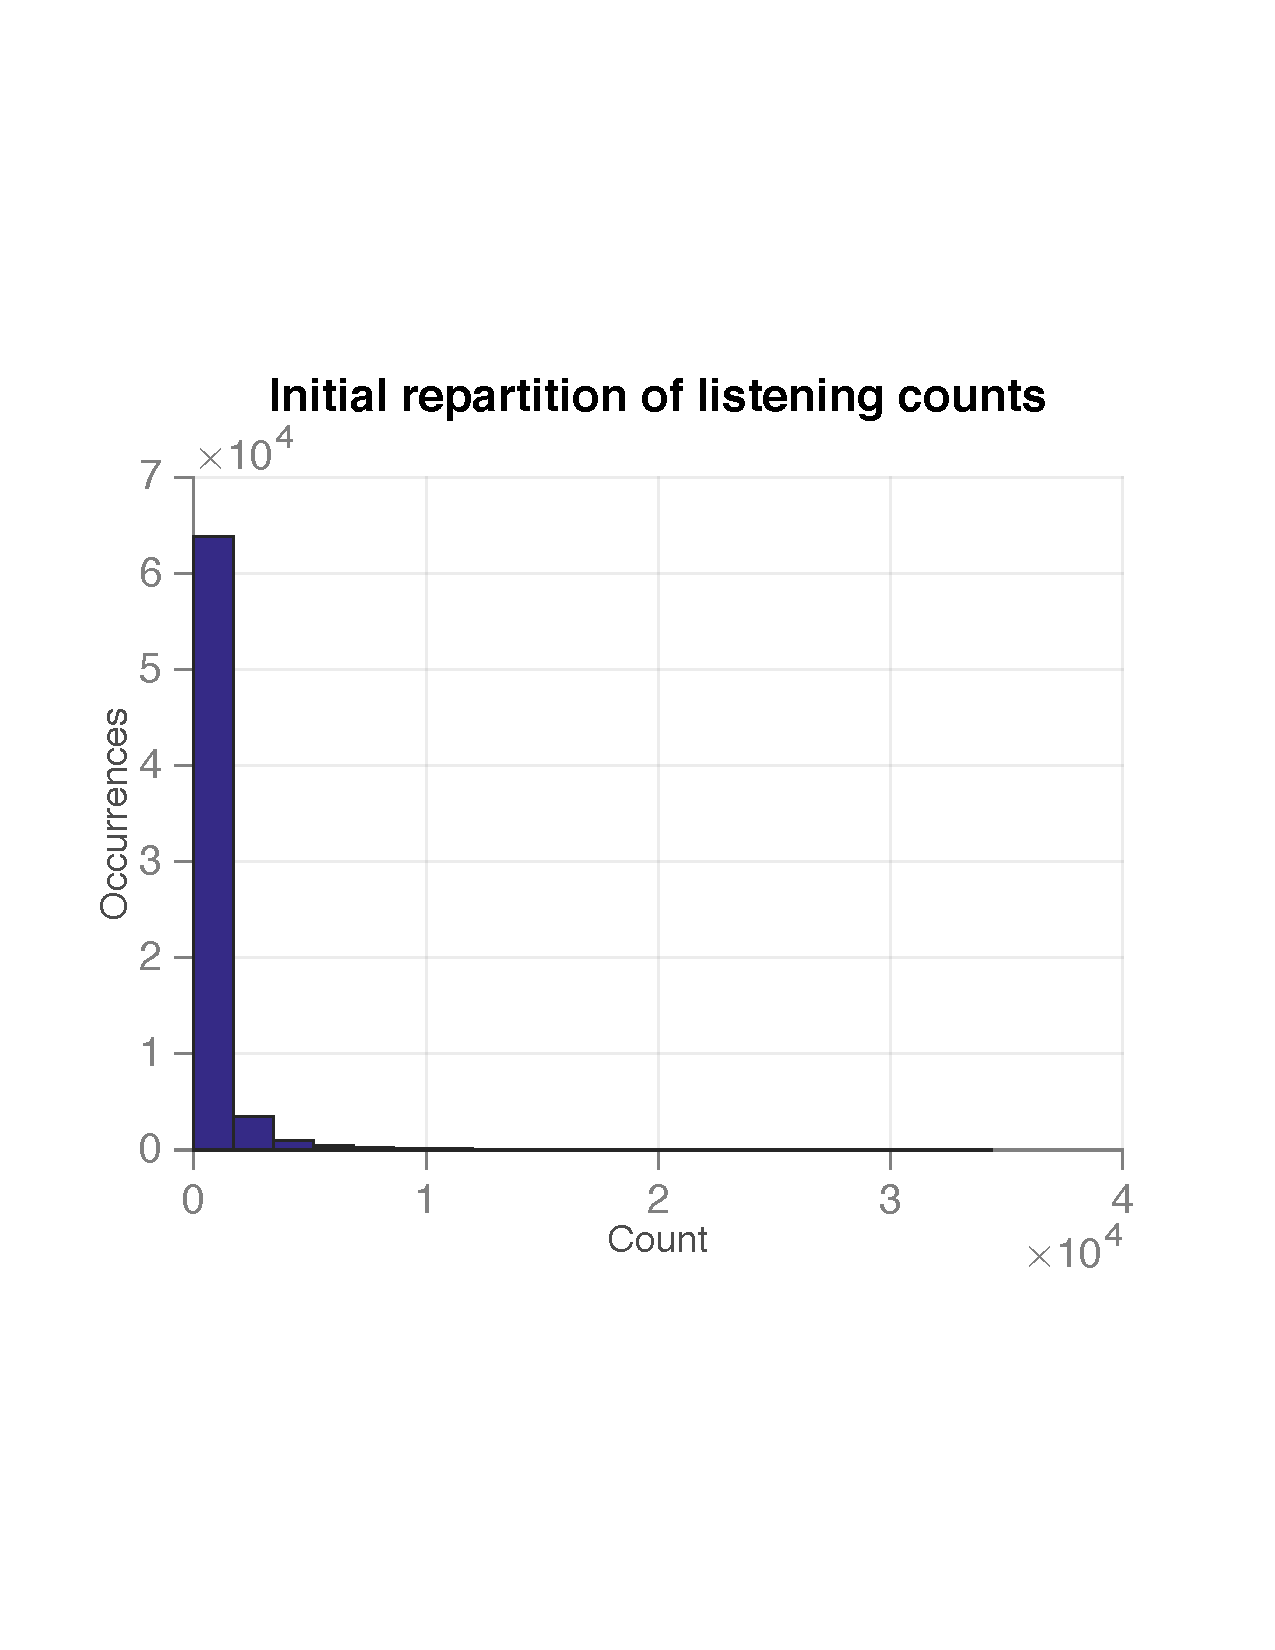
\includegraphics[width=4cm]{figures/recommendation/unnormalized-counts.pdf}
    }
    \subfigure{
      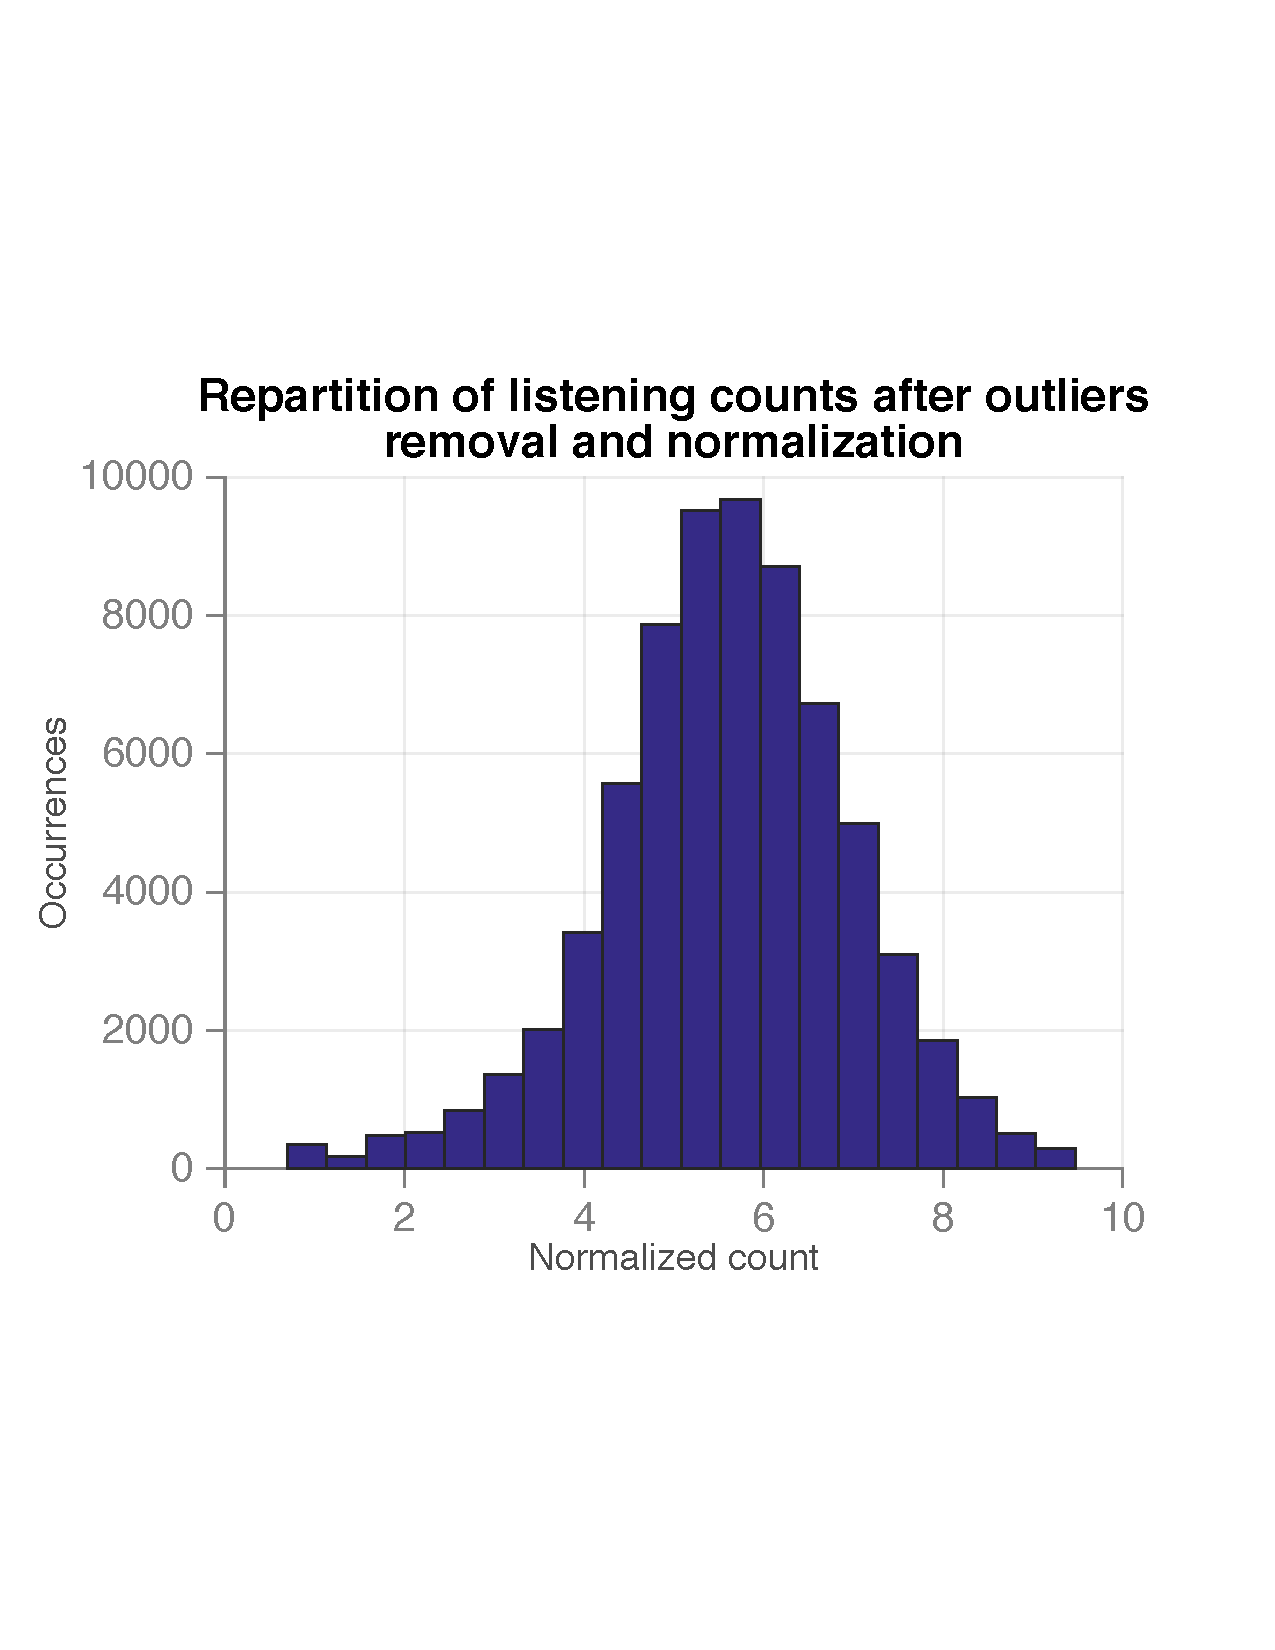
\includegraphics[width=4cm]{figures/recommendation/normalized-counts.pdf}
    }
    \caption{The Quest for Gaussianity}
    \label{fig:recommendation-normalization}
  \end{figure}

  Finally, in order to test our models for both weak and strong predictions, we separated the training set in two ways. We either ntirely remove a proportion of users to use them as a strong prediction test set (typically removed $20\%$). Or we withhold a proportion of the remaining (user, artist, listening count) triplets to use them as a weak prediction test set (typically $20\%$ of the available counts of each user). We use mean \textbf{RMSE} as our main error measure. Given a predicted triplets $\hat{Y}$, we compute the RMSE of the residuals on nonzero elements of the $\log$-transformed target sparse matrix $Y$.

  \subsection{Methodology and baseline}
  We used two baseline predictors to compare our results with: \textsc{OverallMean} which always predict the mean of all observations, and\textsc{MeanPerUser} which always predict the mean of the user. These performed remarkably well, with an expected test RMSE of $1.42$ and $0.867$ respectively. It turns out the latest was hard to beat.\\
  In order to analyze the results of each proposed technique, we rely on three plots: a comparison of the observation's norm versus the predicted norm for each user, a histogram representation of the repartition of errors made for each prediction, and a plot of the mean RMSE per listening count available. This allows us to diagnose the error more precisely than a single RMSE measure (how does the predictor perform when there's a lot of counts available? When there are few? When the counts are large?). Figure \ref{fig:baseline-predictor-plots} shows such plots for the baseline predictor \textsc{MeanPerUser}.

  \begin{figure}[ht]
    \center
      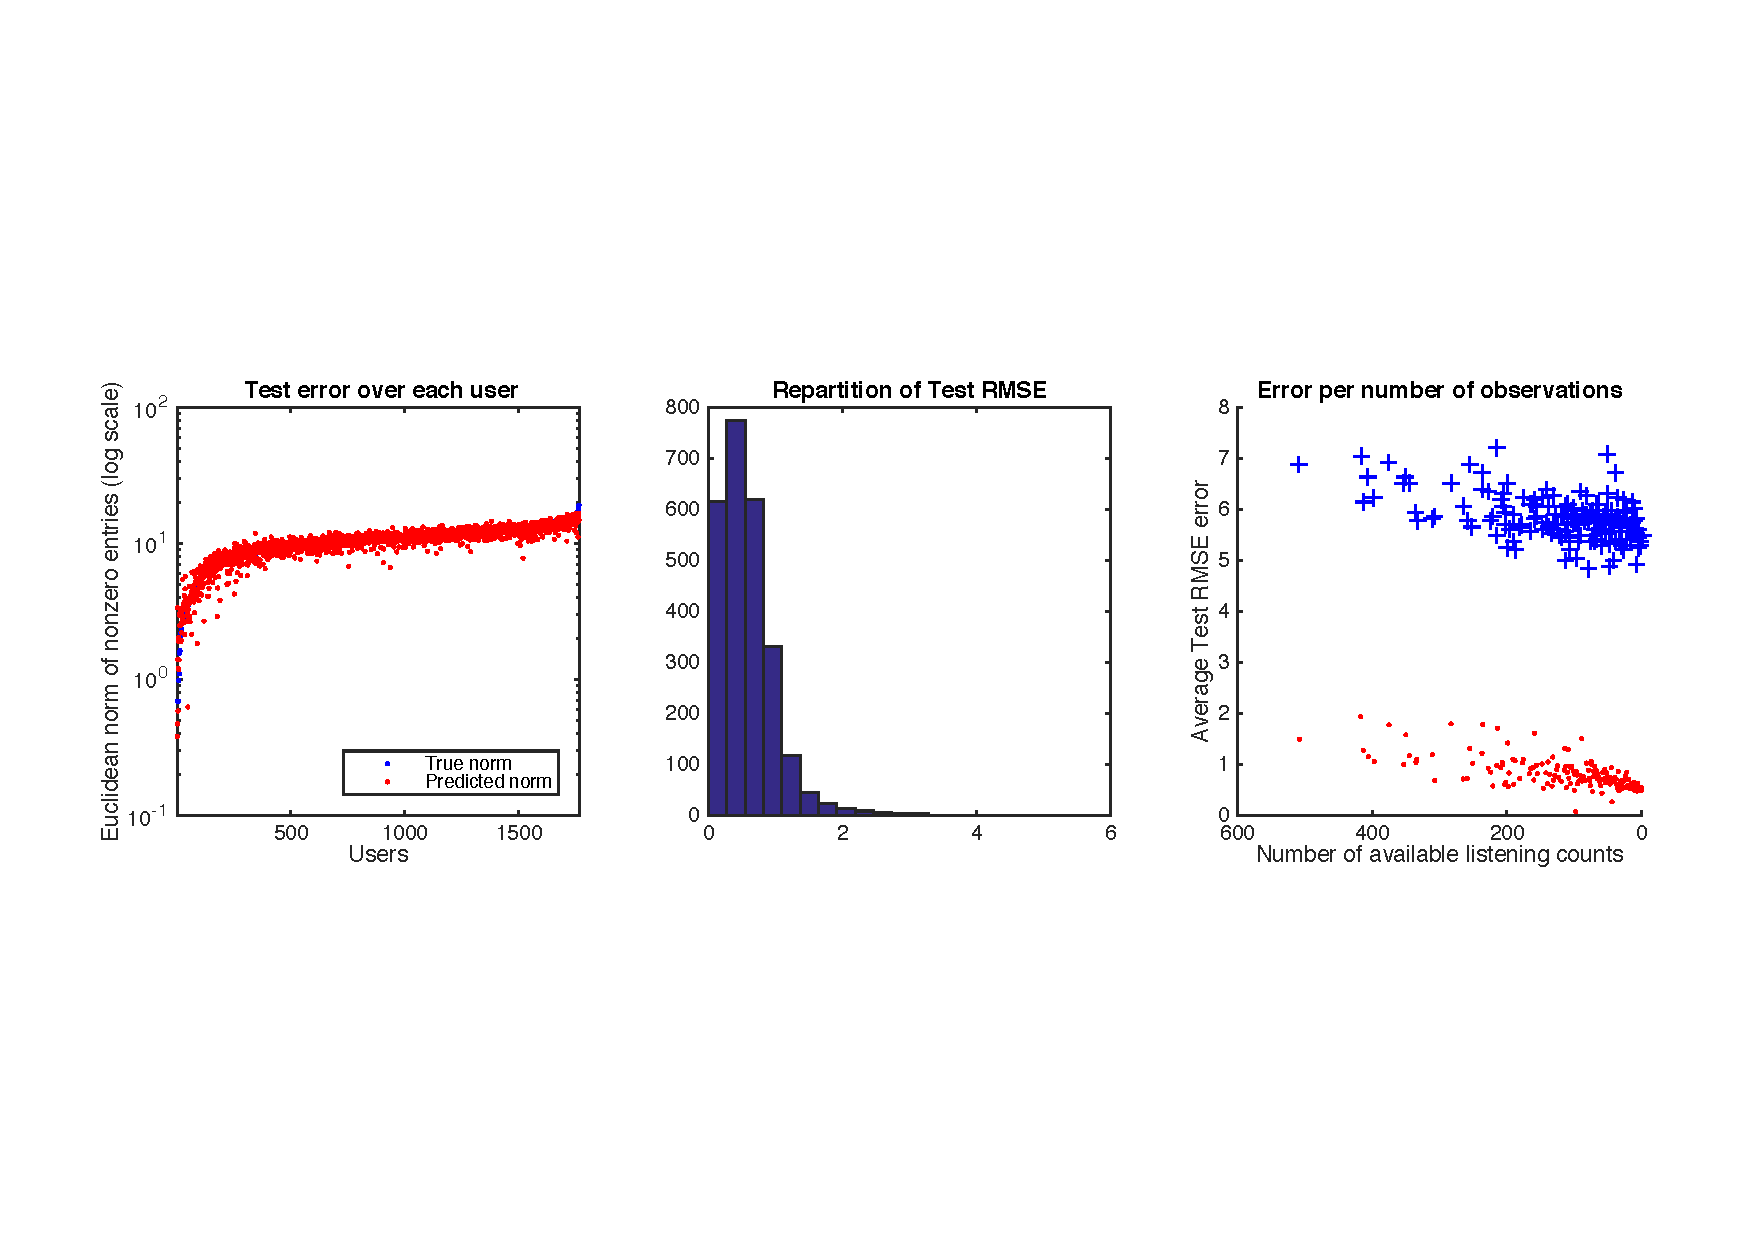
\includegraphics[width=14cm]{figures/recommendation/baseline-predictor-plots.pdf}
    \caption{Error diagnostic for the \textsc{MeanPerUser} baseline predictor. On the right plot, a constant predictor's error is shown in blue for comparison.}
    \label{fig:baseline-predictor-plots}
  \end{figure}


  \subsection{Model-based}
  Model-based approaches to recommender system try to \textit{explain} the observations by training models (e.g. linear regressio) from the observations. However, we are confronted with the classical \textbf{sparsity} and \textbf{long-tail} problems of recommender systems.\\

    \begin{figure}
      \center
        \subfigure[
          \textsc{EachArtist} is not accurate when too few listening counts are observed.
          \label{fig:model-based-predictors-plots:each-artist}
        ]{
          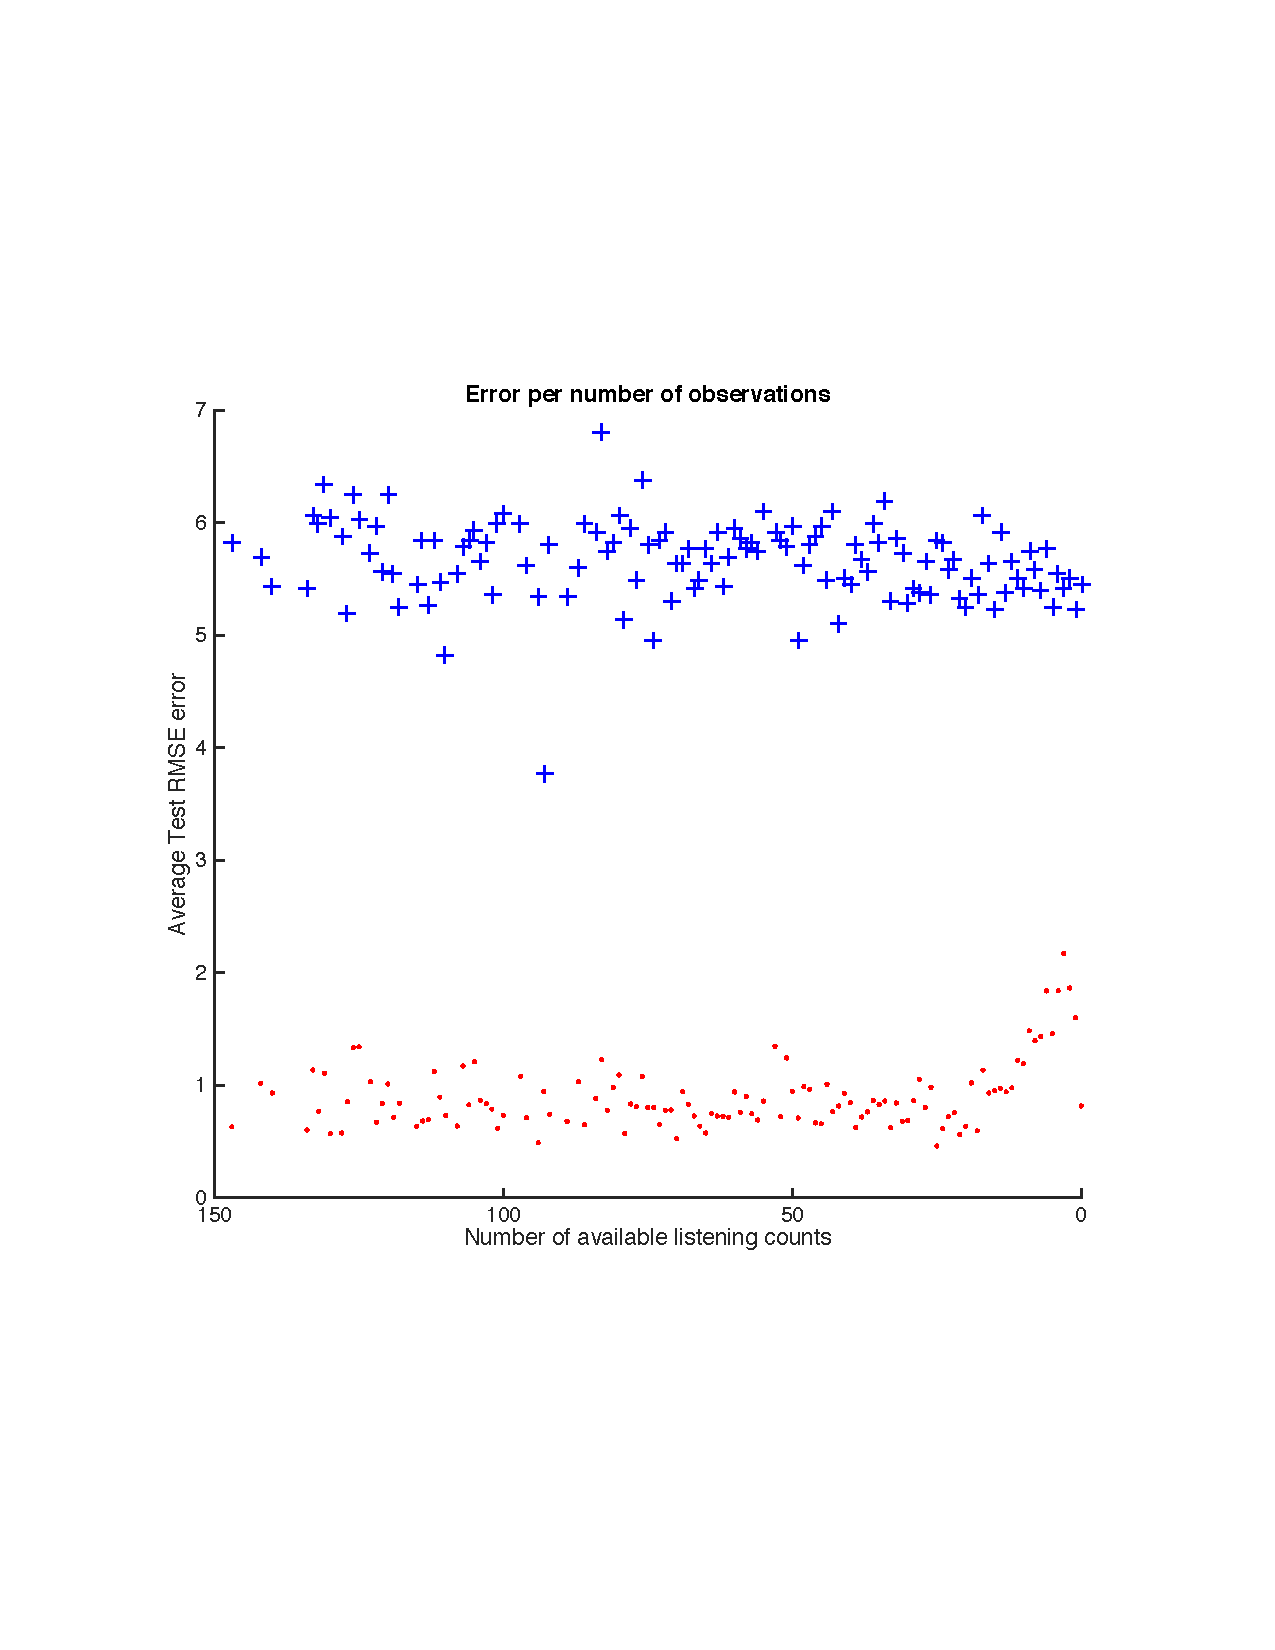
\includegraphics[width=4.5cm]{figures/recommendation/each-artist-predictor-plot.pdf}
        }
        \hfill
        \subfigure[
          \textsc{HeadTailSplit} with cutoff at $10$ and $10$ tail clusters
          \label{fig:model-based-predictors-plots:head-tail}
        ]{
          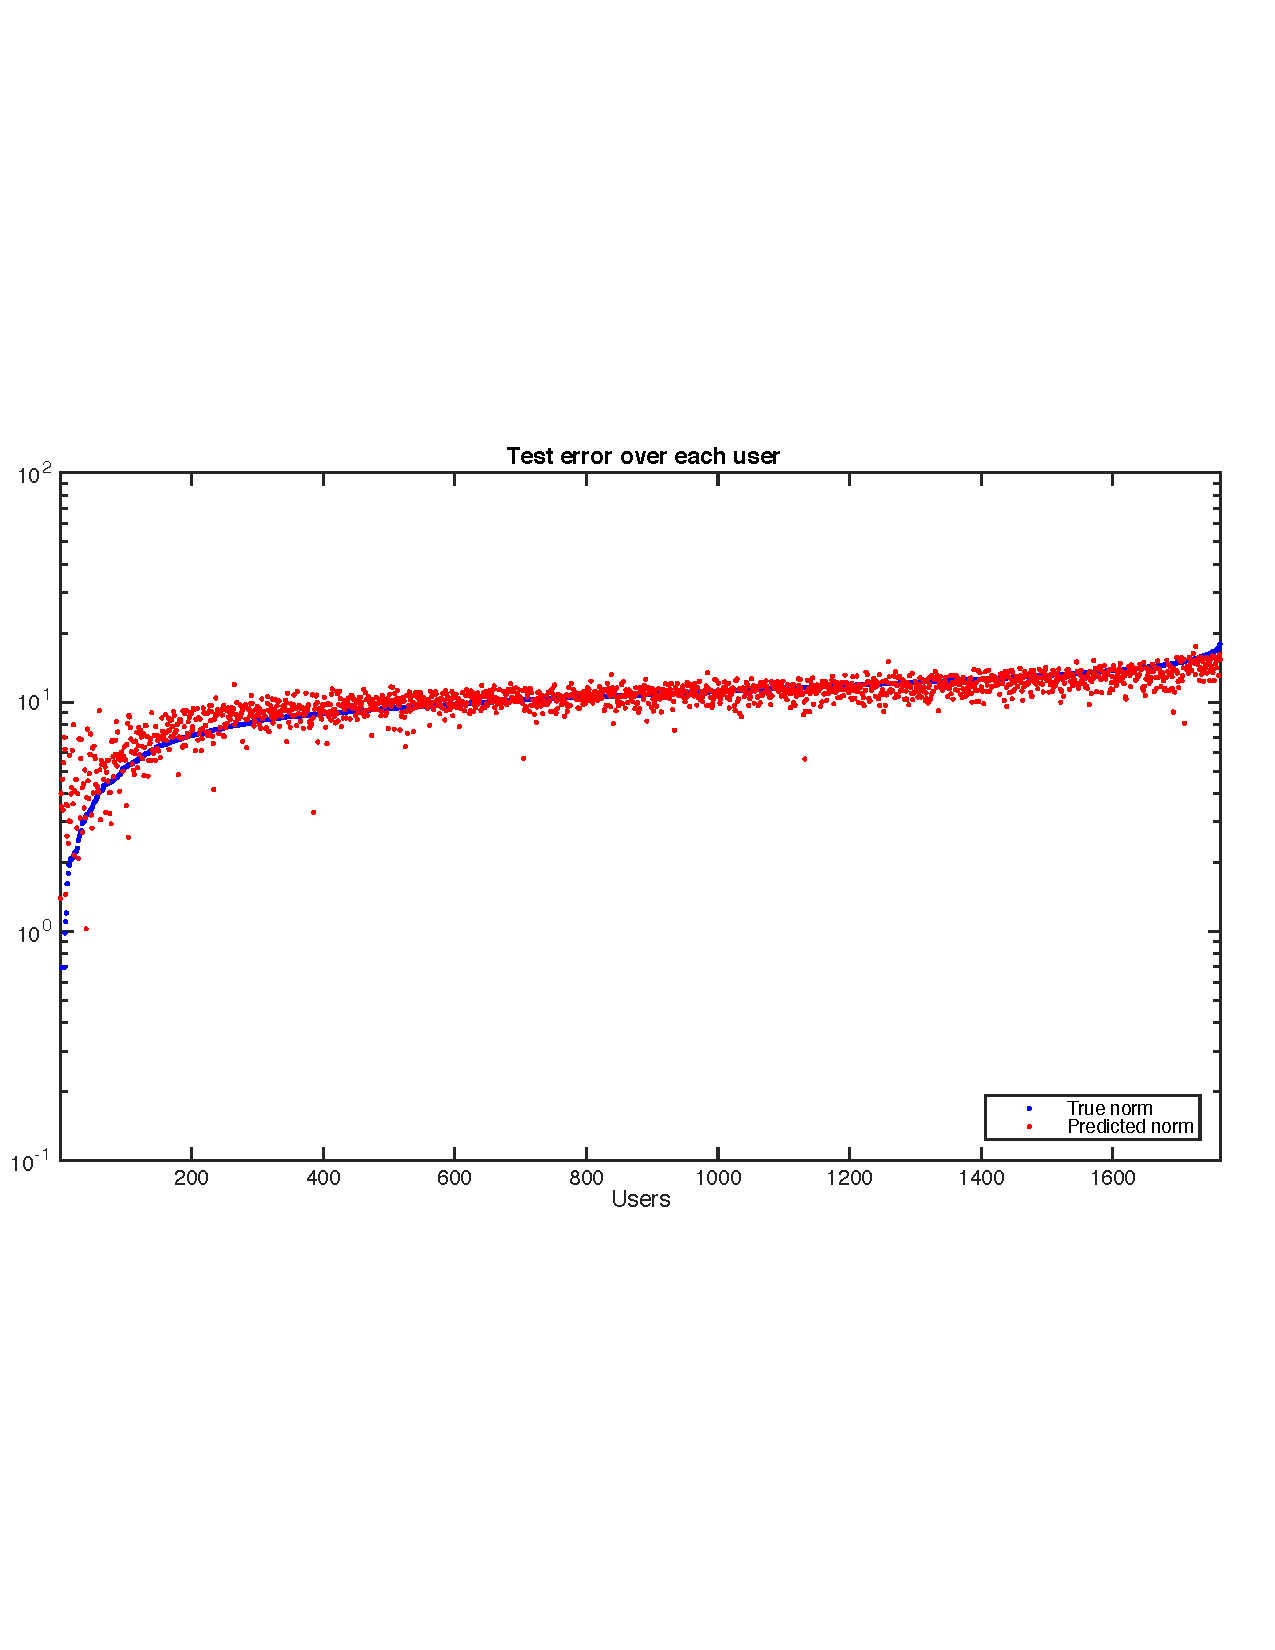
\includegraphics[width=7cm]{figures/recommendation/head-tail-predictor-plot.pdf}
        }
      \caption{Model-based methods}
      \label{fig:model-based-predictors-plots}
    \end{figure}

    \noindent
    \textbf{Each Artist}. We applied an ``item''-oriented approach by training a linear model per artist. The features were extracted as proposed by \cite{long-tail-recommender}, forming a set of Derived Variables (DV) for each user and for each artist. Some of these DVs were also reused in subsequent methods. As shown on figure \ref{fig:model-based-predictors-plots:each-artist}, this approach works fairly well when a large number of counts is available, but fails when data examples are too scarce. \textsc{EachArtist} gives an expected train RMSE of $0.62$, but fails to generalize (test RMSE: $1.41$).

    \noindent
    \textbf{Head-Tail split}. In order to handle better the artists for which very few data points are available (e.g. less than $10$), we follow the method described in \cite{long-tail-recommender}, and split the dataset in head and tail parts. It is important to note that even with a generous cutoff points, a vast majority of the artists lie in the tail of the dataset. While the head can support training a single model (e.g. \textsc{EachArtist}) per artist, tail artists are clustered and used together to learn a common, approximate model. Using a cutoff point of $10$ (minimum number of observations in the Head) and clustering tail items into $10$ clusters, we obtain an expected RMSE of $1.07$. Examining our error diagnostic plots on figure \ref{fig:model-based-predictors-plots:head-tail}, we remark a general tendency to slightly overpredict small entries and underpredict large entries.\\

    \noindent
    \textbf{Low-rank matrix factorization}. We implemented the \textit{Alternating Least-Sqaures with Weighted-$\lambda$-Regularization} (ALS-WR) described in \cite{alswr} to obtain a low-rank representation adapted to our sparse data. It is fast, and our implementation could benefit from easy parallelization. To select the best value of the parameter $\lambda$ ($\lambda \in [10^{-2},10^0]$) as well as the target reduced rank, we run the algorithm with each candidate value over $5$ random train / test splits of our dataset. ALS-WR can fit the training set arbitrarily well, but we were not able to reproduce the good generalization results achieved \cite{alswr} on the Netflix dataset. The best expected test RMSE obtained was $TODO$ (with $\lambda = TODO$ and $TODO$ latent factors). However, we re-used this algorithm in subsequent methods as an efficient dimensionality-reduction tool.

    \begin{figure}
      \center
        \subfigure[Expected train reconstruction error]{
          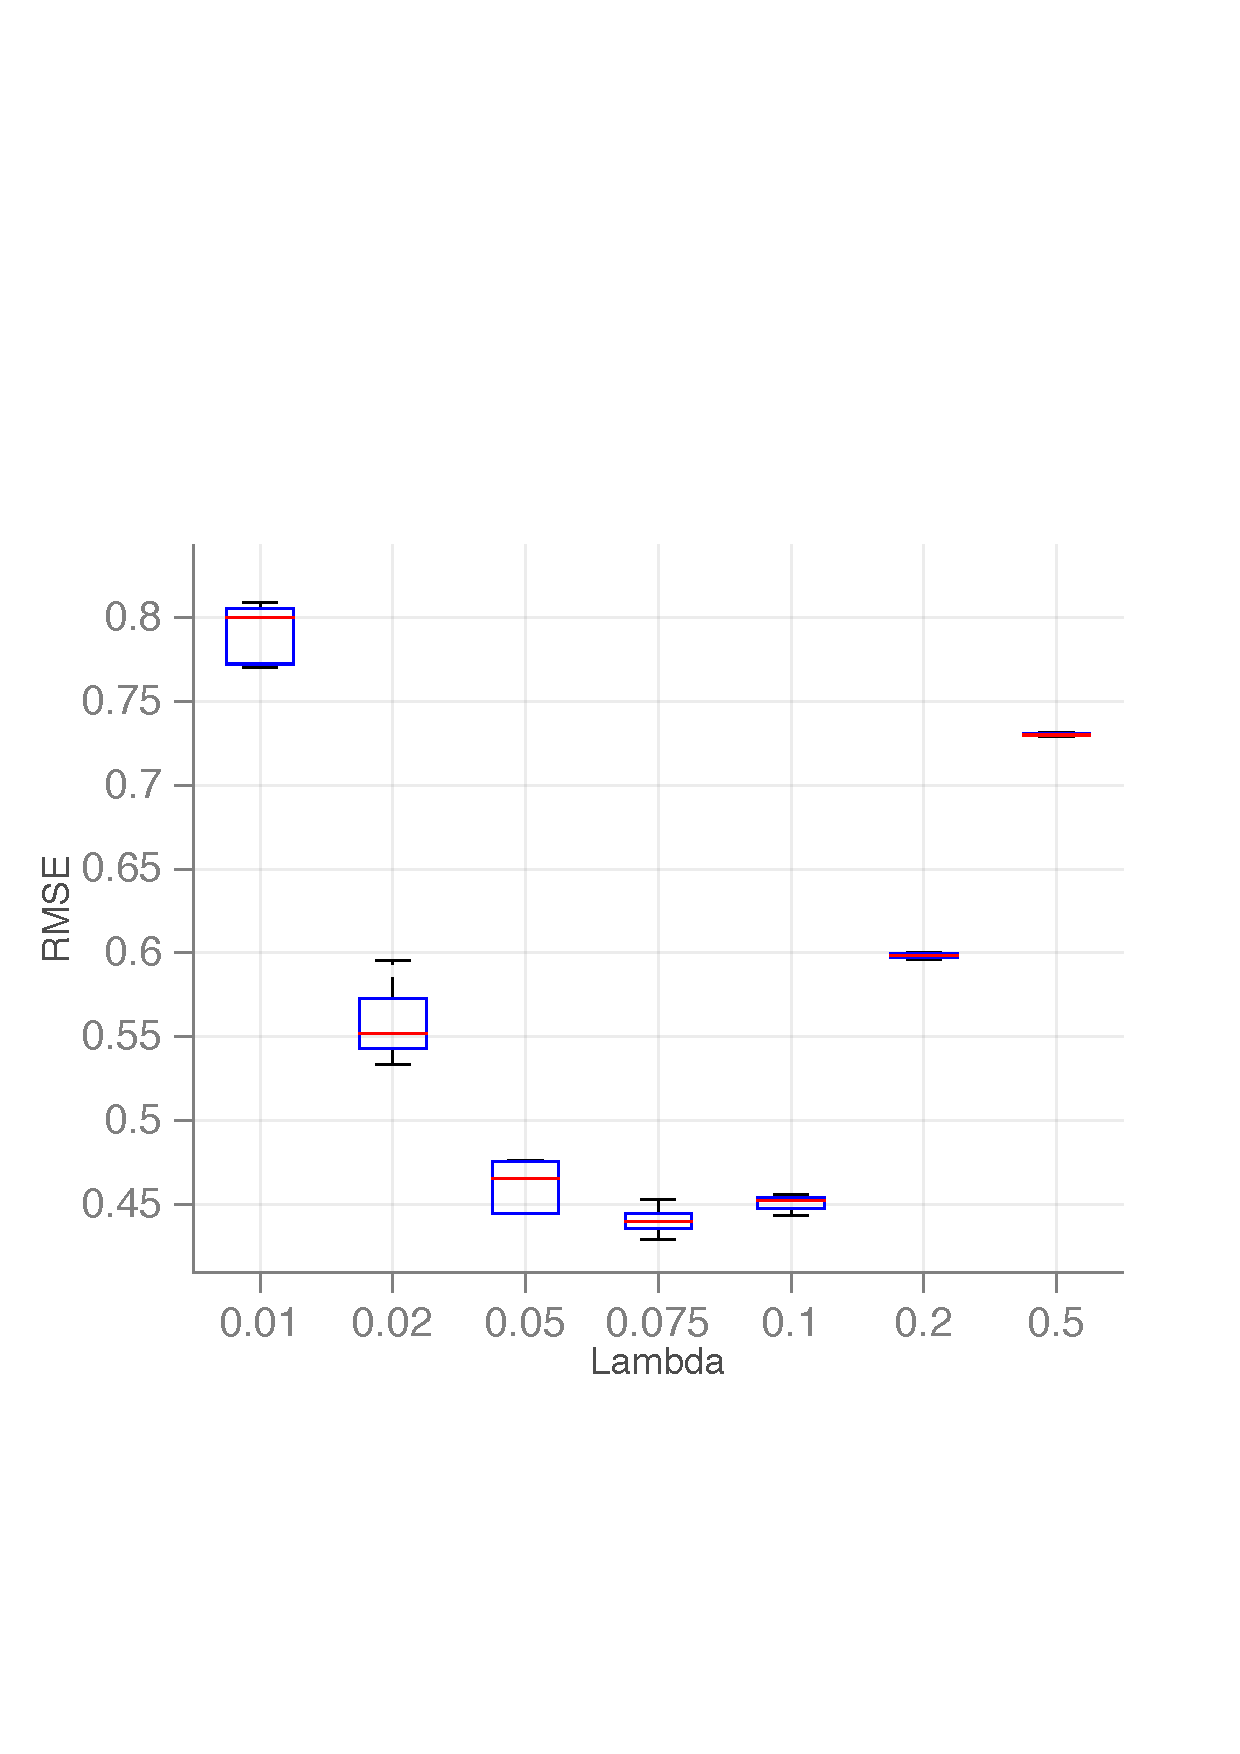
\includegraphics[width=5cm]{figures/recommendation/alswr-lambda-selection-train.pdf}
        }
        \hfill
        \subfigure[Expected test reconstruction error]{
          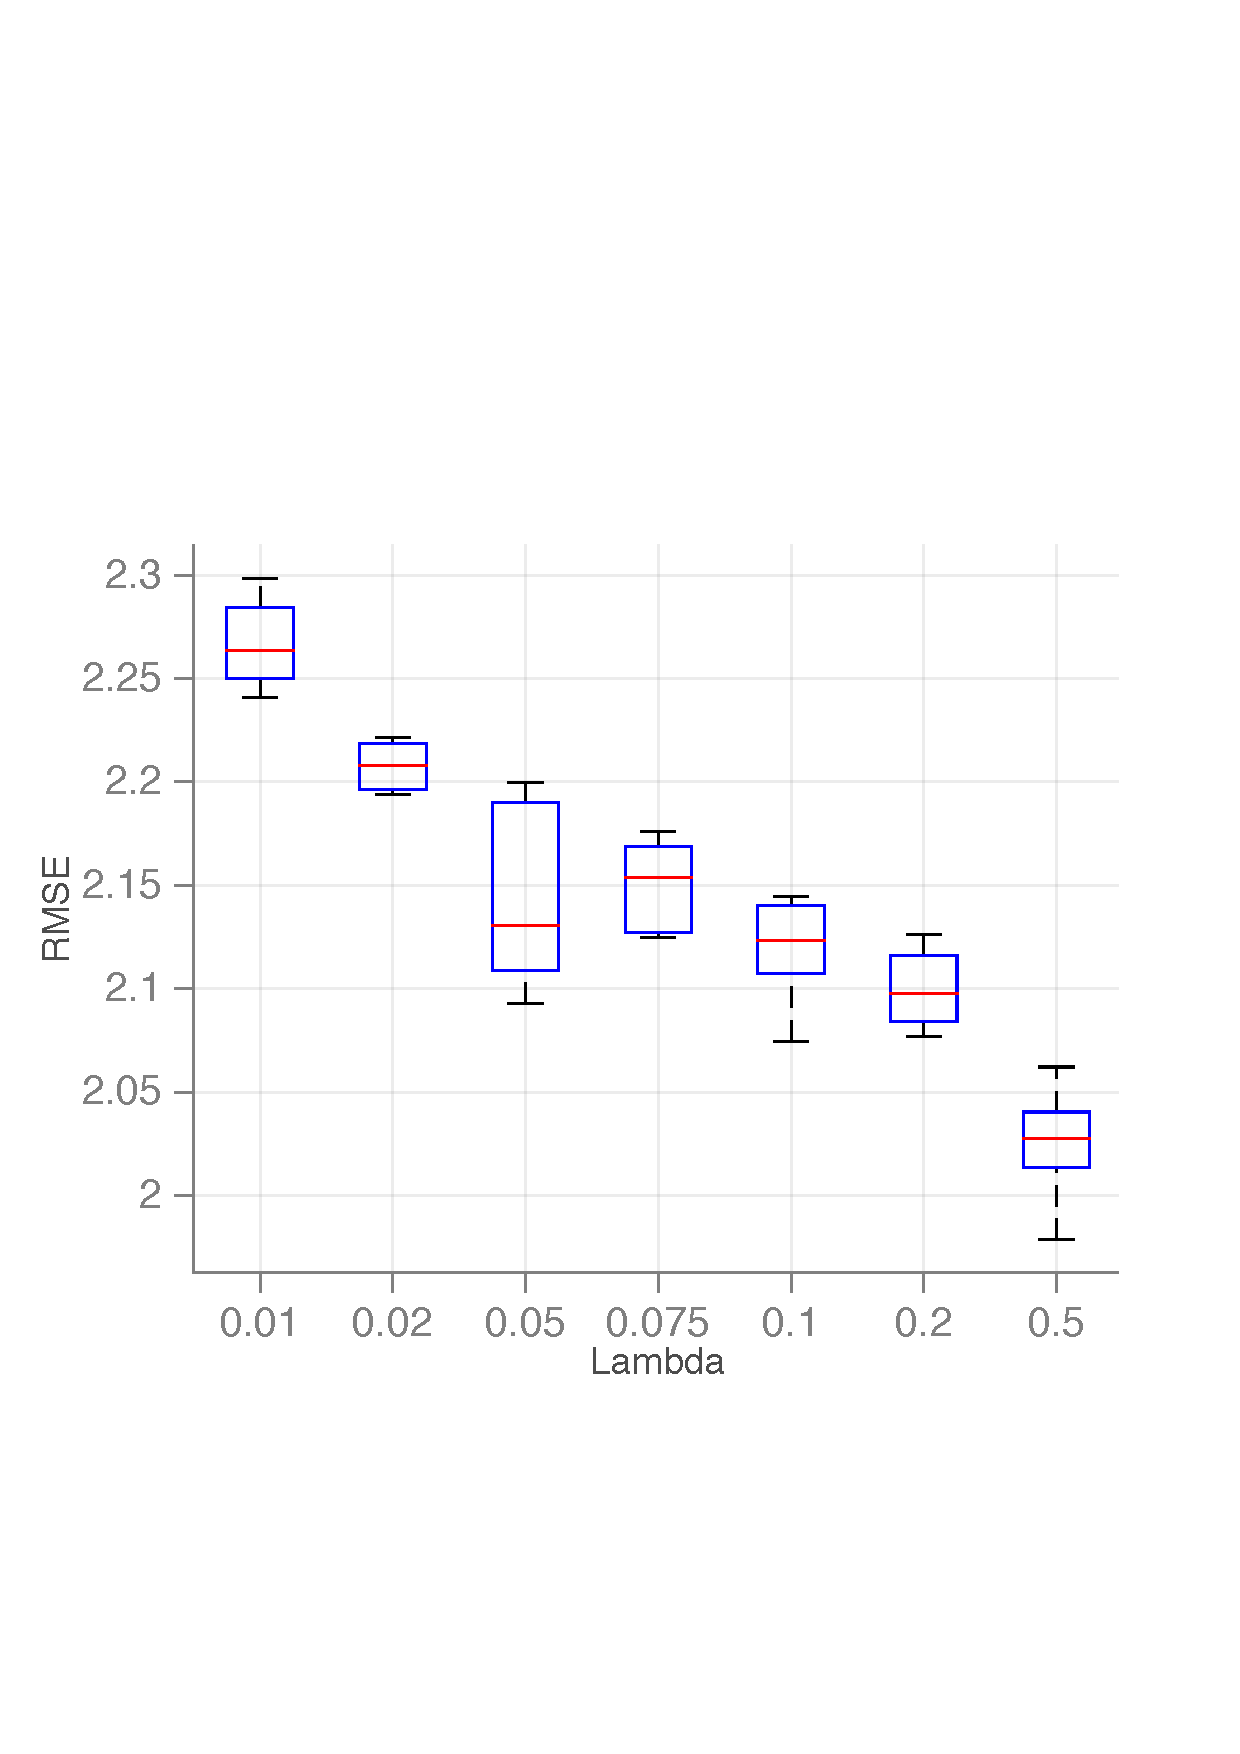
\includegraphics[width=5cm]{figures/recommendation/alswr-lambda-selection-test.pdf}
        }
      \caption{Selection of the $\lambda$ parameter for \textsc{ALS-WR} algorithm with $50$ latent factors.}
      \label{fig:model-based-predictors-plots}
    \end{figure}

  \subsection{Memory-based}
  Memory-based approaches, as opposed to model-based, do not rely on the semantics of the data. On the other hand, we make the assumption that people have stable \textit{tastes} or preferences, that is that users who agreed in the past will agree in the future and that they will like similar artists than those they listened to in the past. While this approach may show limitations on large temporal scale, it proved successful on our dataset.\\

    \noindent
    \textbf{K-means clustering}. Intuitively, grouping the users by taste would allow us to generate generic profiles and use them for prediction. The simplest approach is the classical K-means algorithm and predict the cluster's centroid. Since the Euclidian distance measure tends to become less meaningful in high dimensional space (related to the curse of dimensionality), we used the Cosine metric to compare users and group them into clusters. We used the fast \texttt{kmeans2} implementation provided by \cite{piotrtoolbox}.\\
    Even when increasing the number of clusters, simple centroid prediction failed to generalize and never achieved (in our tests) a better test error than the baseline. This clustering method can however be extended beyond centroid prediction, as we show next.

    \noindent
    \textbf{Gaussian Mixture Models} with Expectation Maximization (EM) for soft clustering: K-means has the disadvantage of producing ``hard'' cluster assignments. Gaussian Mixture Models, on the other hand, yield ``soft'' clustering, enabling us to capture more nuanced profiles. \cite{gaussian-mixture-model-script} provides an EM implementation relying on Variational Bayesian Inference to choose automatically the most appropriate number of clusters, effectively minimizing the number of hyperparameters to select.\\
    However, the algorithm had computational requirements too large for our time constraints, and so we decided to cluster users \textbf{after projection} on a lower dimensional space. Using a low-rank approximation to cluster on also has the advantage ofreducing overfitting. We used our ALS-WR implementation to generate this low dimensionality approximation of the users, and obtain soft cluster assignments in that space. We then predict the reconstructed counts $\hat Y$ (as described in \cite{alswr}), weighted by the soft assignment coefficients. Without precise parameter tuning, we obtain $TODO$ RMSE, which is in fact consistent with the performance obtained with ALS-WR.\\

    \noindent
    \textbf{Top-N similar users}. Our best results were obtained by basing our predictions on a user similarity measure. We selected the \textbf{Pearson product-moment correlation} coefficient as described in \cite{cf-techniques-review}. For two users $i$ and $j$, we compute their similarity as:
    \[
      \text{similarity}(i, j) = \frac{
        \sum_{k \in \text{common artists}} (r_{ik} - \bar r_{i})(r_{jk} - \bar r_{j})
      }{
        \sqrt{ \sum_{i\text{'s counts } r_{ik}} (r_{ik} - \bar r_{i}) }
        \sqrt{ \sum_{j\text{'s counts } r_{jk}} (r_{jk} - \bar r_{j}) }
      }
    \]
    where $\bar r_i$ is the average listening count of user $i$ and $r_{ik}$ is the listening count of user $i$ for artist $k$. Intuitively, the terms involving a deviation to the user's mean encode preference. It also allows to ignore the large variations in listening habits (small and large volume users). Since the sum in the nominator only takes into account artists which both users have listened to, users with no artists in common have a similarity of $0$. On the other hand, users having listened to exactly the same artists will have either $1$ or $-1$ similarity, based on whether or not they ``liked'' it (i.e. if they listened to it more or less than to other artists).

    The \textsc{Top-N-Neighbors} predictor selects the $N$ most similar users and predicts based on their ``vote'', that is their listening count minus their average listening count. We add a biais term $\bar r_i$ to account for the current user's listening habits. The predicted listening count of user $i$ for artist $j$ is then:
    \[
      \hat r_{i,j} =
        {\bar r_i} +
        \sum_{u \in \text{~Top N neighbors}}
          k \times \text{similarity}(u, j) \times (r_{uj} - \bar r_{u})
    \]

    Computing the similarity coefficient proved somewhat costly. For very large datasets, as for the clustering techniques, it is possible to use a low rank approximation of the dataset to compute the correlation coefficients on. The Top-N predictor's hyperparameters ($N$ and the space to compute the similarity in) can be tuned to strike a balance between prediction quality and computation time.

    \noindent
    \textbf{Final model and predictions}. Since the number of users remains limited ($\leq 2000$), we were able to fully compute the similarity matrix $S$ on the training data and predict using the votes of \textit{all} other users. To make it possible in reasonable time, we implemented a parallelized similarity matrix computation function. Figure \ref{fig:similarity-predictor-plots} shows the error diagnostic for this method. We obtain an expected test RMSE of $0.76$, which finally beats the \textsc{MeanPerUser} baseline. We researched further processing which could be applied to the similarity matrix, e.g. Fisher's $z$ transform, but it didn't seem to improve the results.

    \begin{figure}[ht]
      \center
        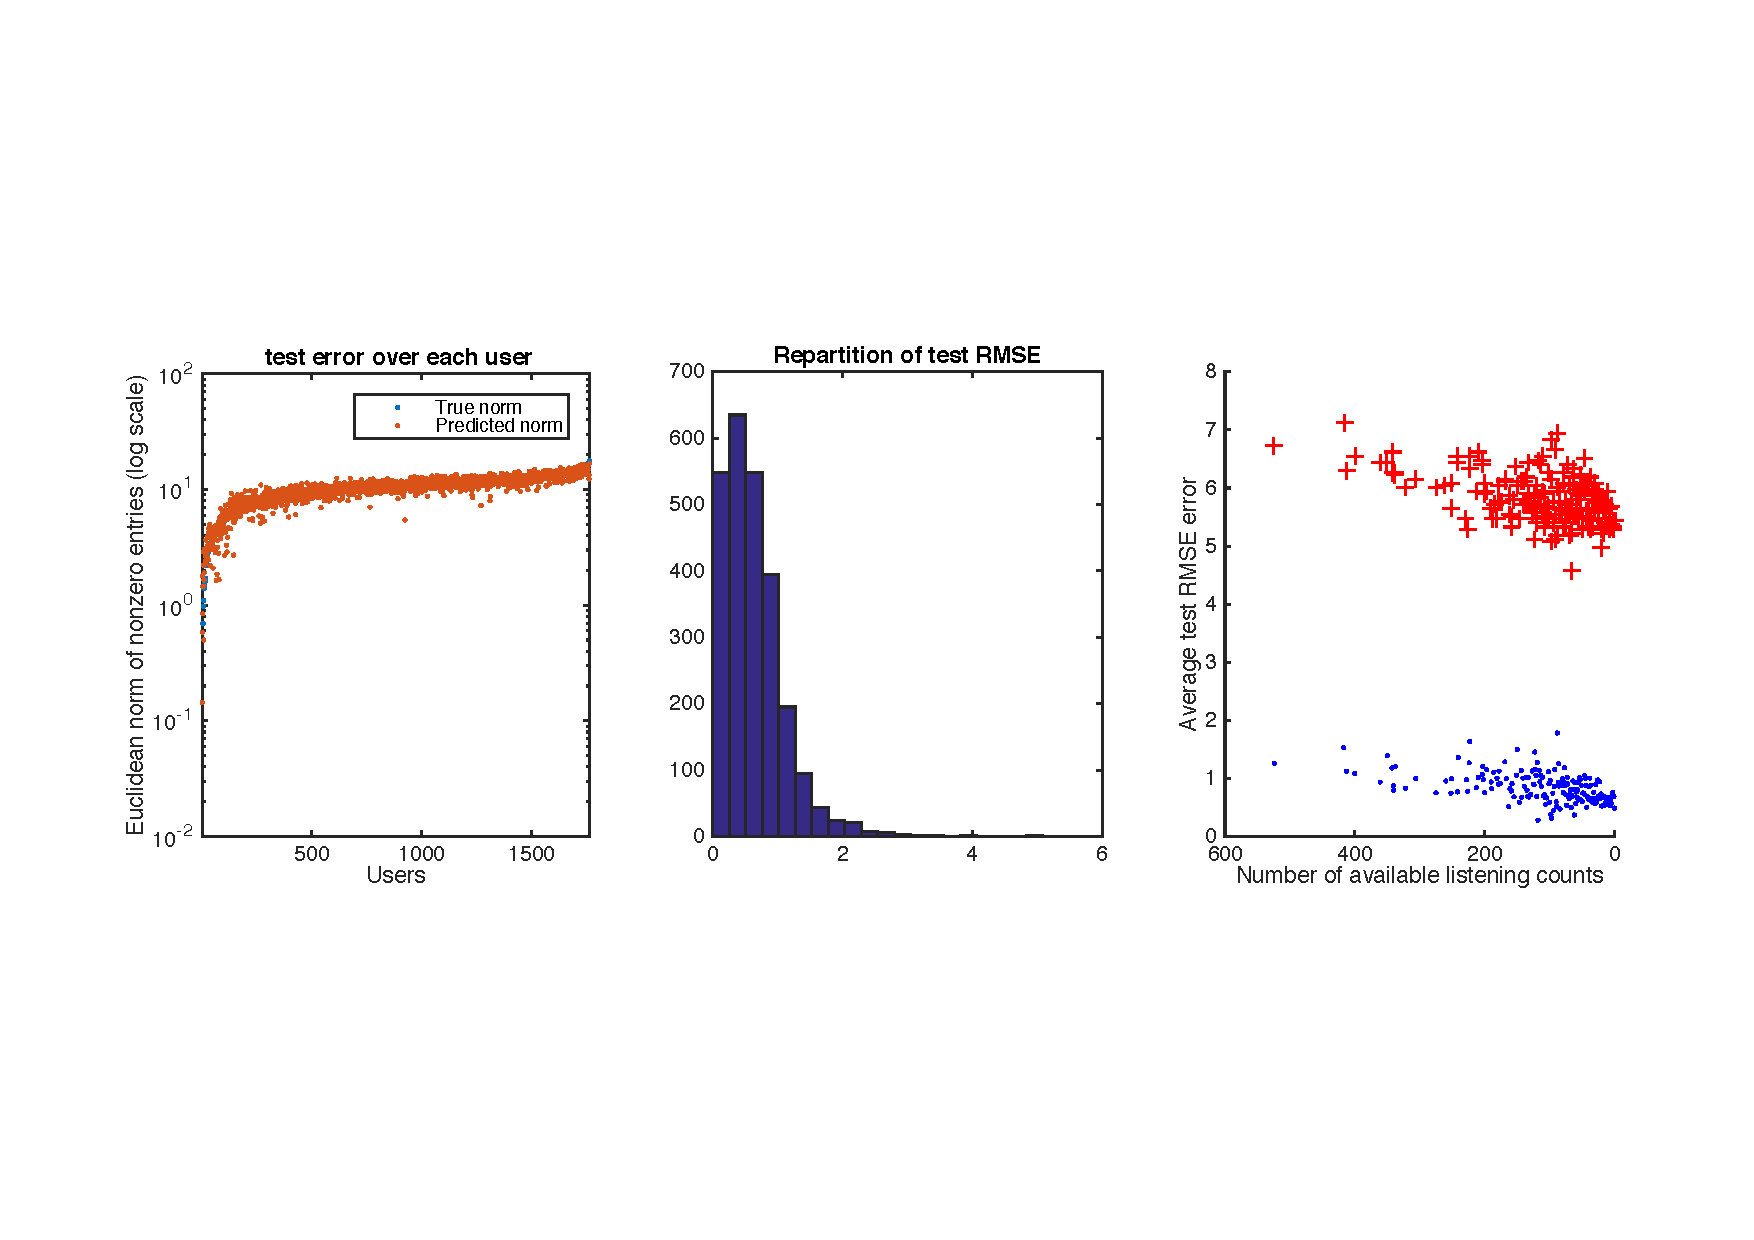
\includegraphics[width=12cm]{figures/recommendation/similarity-predictor-plots.pdf}
      \caption{Error diagnostic for the \textsc{Similarity} predictor}
      \label{fig:similarity-predictor-plots}
    \end{figure}


  \subsection{Strong generalization}
  In the strong generalization task, the baseline is to predict the overall mean of all counts and achieves an expected RMSE of $1.44$. Given the very little information available to generate predictions, even a minor improvement over the baseline seems satisfactory. One of the largest factor of error is that we do not know if the new user will have large or small listening counts. We estimate its mean listening count as the median of all available mean listening counts, which corresponds to the assumption that this user will behave similarly than a majority.\\
  We tried using the friendship graph data to our advantage by encoding the following assumptions in our predictions: a user has tastes similar to its friends'; a heavy user is friend with heavy users (resp. light). Unfortunately, they didn't seem to correspond to the observations, since the expected RMSE never consistently beat the baseline. We were not able to extract signal from the friendship graph.\\
  However, we did achieve a small improvement by using a measure of ``likeability'' of artists. We define likeability as the mean deviation of listening counts received to their respective users' mean. However, this measure only makes sense when some amount of observations are available (otherwise, we replace it by $0$). We estimate the unknown user's mean as described above. With these simple manipulations, we obtain an expected RMSE for strong prediction of $1.39$, which is slightly below the baseline.

  \subsection{Further work}
  ``Cold start'' and recommender systems in general are an active area of research. We noticed several promising techniques in the litterature, such as Slope One (\cite{slope-one}) for weak generalization or the use of Boltzman machines for cold start (\cite{cold-start-metrics}). Moreover, the head-tail splitting technique could have been exploited further and combined with more advanced clustering and prediction techniques. Finally, information conveyed by the social graph should be used (\cite{top-k-with-social-network}).

\section{Image classification}

  \subsection{Dataset description}
  \textbf{Objective}: The people detection dataset consists of a set of images associated with a label that indicates whether there is a person or not in the image. Our goal is to predict whether people are present in unseen images.

  \textbf{Data characteristics}: The training set is composed of $8545$ examples. For each of these images, we are provided with the Histogram of Oriented Gradient (HOG) features, generated with Piotr's toolbox \cite{piotrtoolbox}. Hence for each image we convert the features into a vector of dimensionality $9360$. The training dataset includes $1237$ positive examples (images with a person on it) encoded with the label $+1$ and $7308$ negative examples encoded with the label $-1$. The distribution is thus heavily skewed towards negative examples. The test set that we have to make predictions for is composed of $8743$ examples.

  \subsection{Performance Evaluation}
  As our dataset is imbalanced, we are relying on both True Positive (TP) and False Positive (FP) values as indicators of our performance. We are using the Receiver Operating Characteristics (ROC) measure and associated \textbf{ROC curves} to compare and evaluate our classifiers' performances. The ideal working point is the top-left corner of the ROC curve, where no misclassification is made (as explained in \cite{rocanalysis}) .

  \subsection{Dataset pre-processing}
  From data exploratory analysis, we did not spot any obvious outlier. For all features, the examples of the training dataset lie between 2 and 3 standard deviations from the median. \\We tried several feature transformations: $\log$, $\exp$, $\sqrt{.}$ and $.^2$ of the input features. The $\exp$ transformed data associated with a Principal Component Analysis seems to enhance performance so we decided to apply it before reducing the data with PCA and working with these new features, otherwise we keep the original features when working with the full-dimensionality matrix. \\We normalized our features before using them for training.

  \subsection{Principal Component Analysis}
  Our features matrix is of dimensionality $9360$ for $8545$ examples which gives us a "fat'' matrix. As several Machine Learning algorithms' time complexity grows fast with dimensionality, we applied a Principal Component Analysis (PCA) in order to work with lower dimensionality data. To do so, we used Piotr's \texttt{pca} implementation which proved to be faster than Matlab's default implementation. We experimented different rank approximations (keeping $50$, $75$, $100$, $300$, $500$ and $1000$ principal components) and applied a simple logistic regression with 3-fold cross validation to have an heuristic about the performance. From the analysis of the resulting ROC curve averaged over the folds \ref{fig:detection-pca-roc-curve}, we decided to keep $100$ principal components for our data projection. Let call $X_{pca}$ the resulting reduced input features.

  Using a reduced number of features also helps avoiding overfitting, as we are, to some extend, using only the signal (residing in the principal components). We have almost $50\%$ of the variance explained in our reduced space \ref{fig:detection-pca-variance}, the rest being mostly noise.

   \begin{figure}[ht]
       \center
      	\subfigure[ROC Curve of logistic regression applied to different low-rank approximation.]{
      		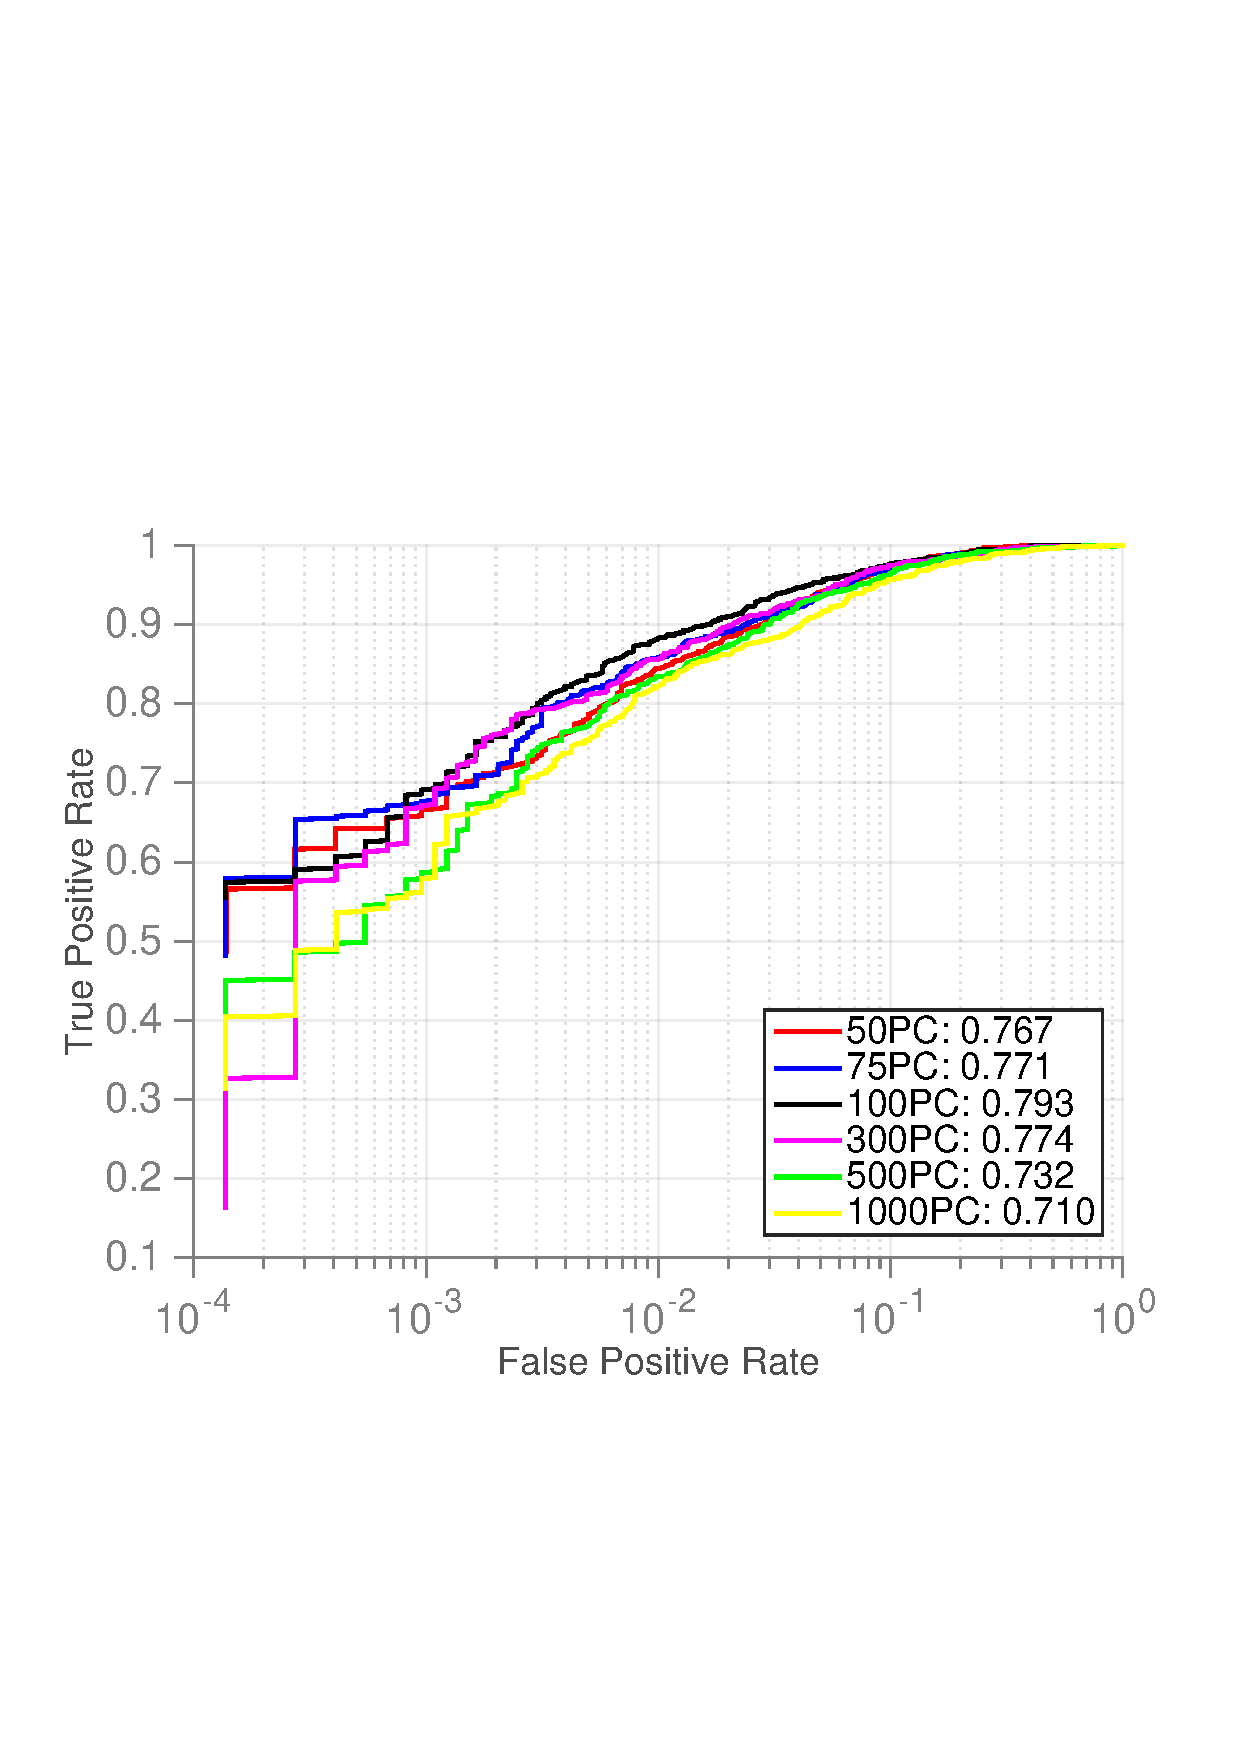
\includegraphics[width=2.5in]{figures/detection/pcaselection-curve3.pdf}
      		\label{fig:detection-pca-roc-curve}
      	}
    	\hfill
	\subfigure[Explained variance per principal component (barplot) and cumulated explained variance (curve).]{
      		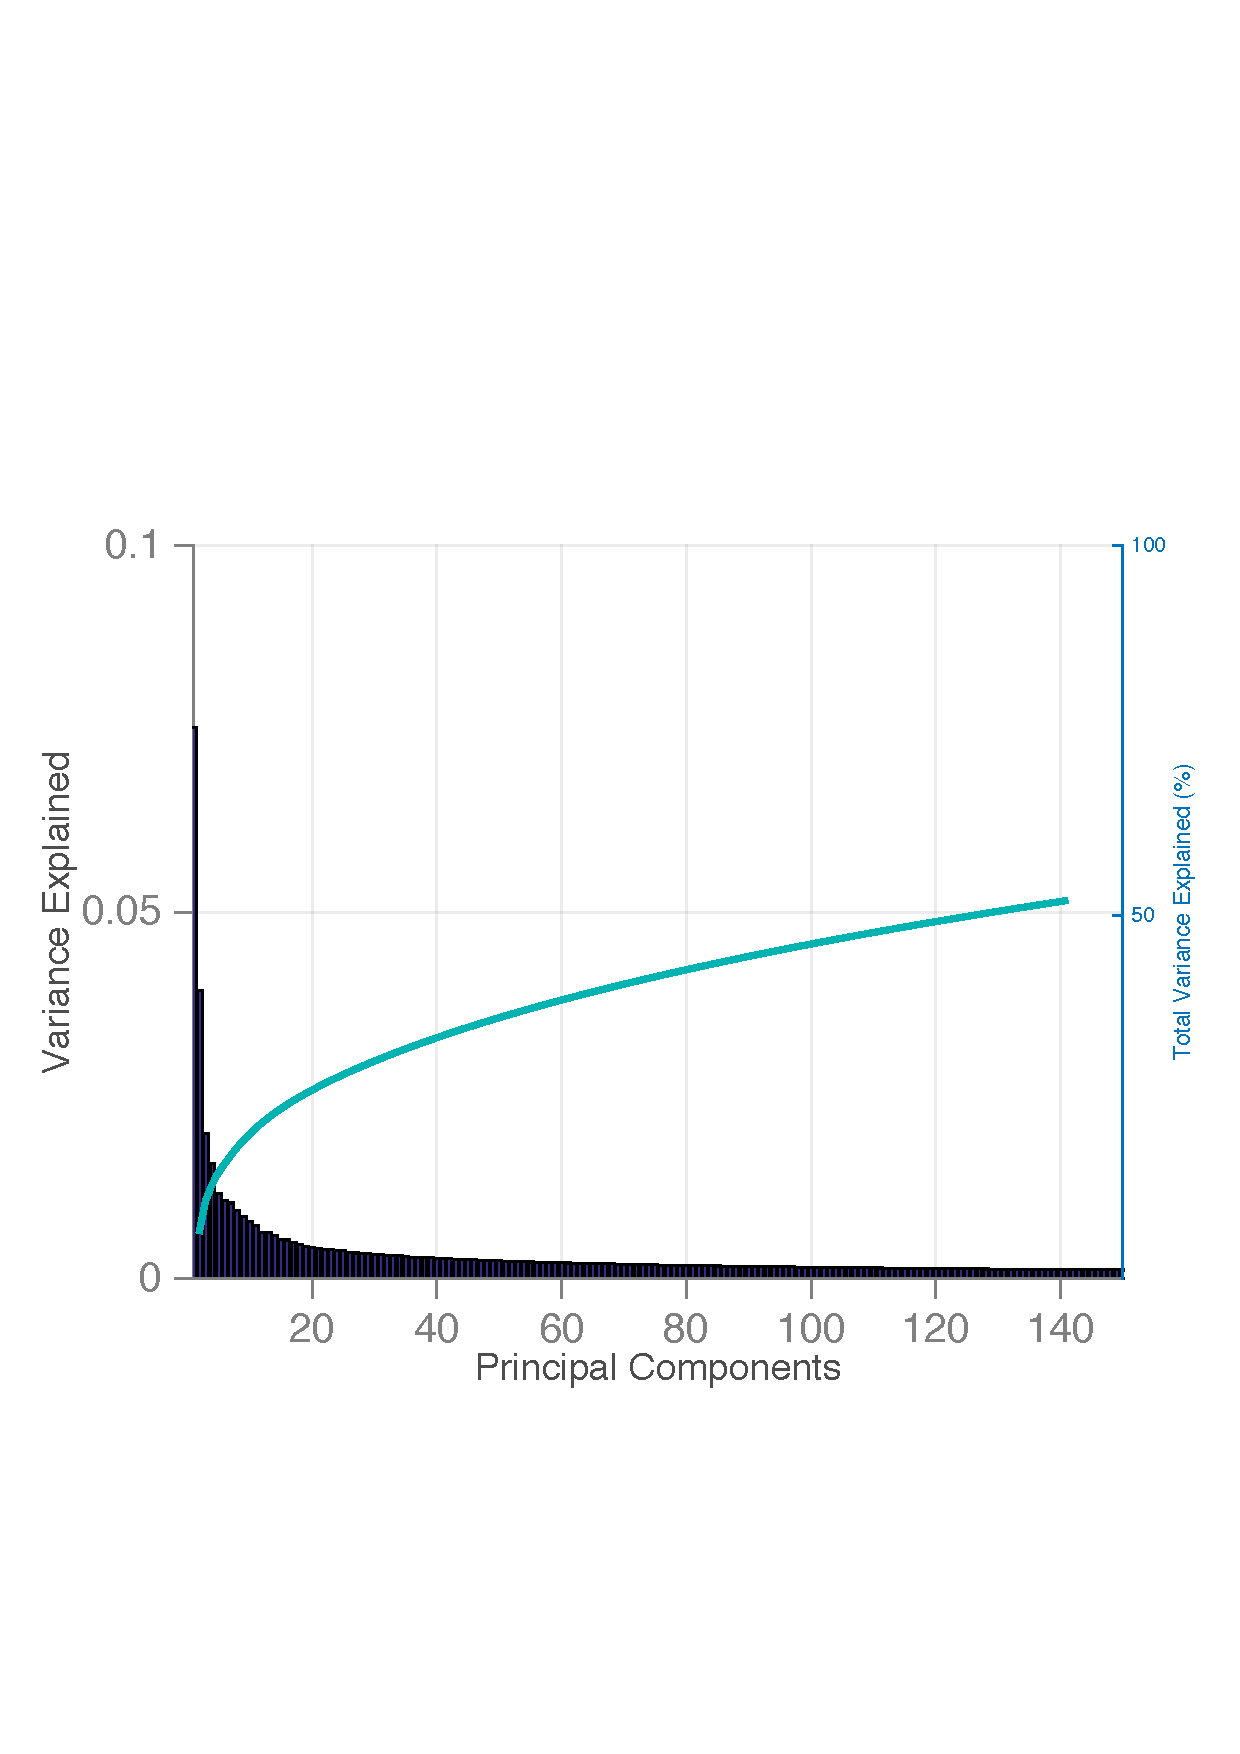
\includegraphics[width=2.5in]{figures/detection/pca-varianceExplained.pdf}
      		\label{fig:detection-pca-variance}
    	}
	\caption{PCA on detection dataset. Selection of the number of principal components}
  \end{figure}

  \subsection{Training different classifiers}
  We learnt classifiers from several supervised learning techniques and compared them to find the best performing model. We started with a simple Logistic Regression. Then, we applied Gaussian Processes classification using Rasmussen's GPML library \cite{gpmltoolbox},  Neural Networks with the Deep Learning toolbox \cite{deeplearningtoolbox}, Random Forests using Matlab's implementation and finally Support Vector Machines using LIBSVM toolbox \cite{libsvmtoolbox}.

  \textbf{General Approach}:
   	\begin{itemize}
	   	\item Applying a default implementation of the model to normalized input data or to $X_{pca}$ depending on computation complexity and performance of the algorithm.
    		\item Tuning model parameters: for parameters that seemed relevant, we chose a range of values to test on and find the best combination using cross validation. As training the different models is rather slow, we used 3-fold cross validation. Other parameters were set manually. We plot averaged performances curves over the range of parameters and select parameters values that maximize the average True Positive Rate (TPR) on the test set. It is important to point out that we may not select the very best parameter doing so because the average TPR is only a proxy however it is the only measure we can rely on to automate the search.
		  \item Validating the trained model using 3-fold cross-validation: we computed an average ROC curve over train and test data. We represent the curve with its 95\% confidence interval.
	\end{itemize}

  \textbf{Logistic Regression}: Since it can be seen as a single-layer Neural Network, we used the Deep Learning toolbox. We applied this classifier on $X_{pca}$ and learnt the regularization term (see below for details) with cross validation and ended up with a regularization term of value equal to $10^{-3}$.

  \textbf{Gaussian Processes}: Having a large number of data examples in our training set, we used "large scale'' GP classification. It relies on low-rank and diagonal approximation to the exact covariance using induction points. Solving a classification problem, we opted for a logistic function as a likelihood function. We did not have specific intuition about the prior distribution so we used a constant 0-mean prior. We selected a squared exponential covariance with isometric distance measure \texttt{covSEiso} rather than the ARD one. While yielding comparable performance, the former uses only two hyper-parameters, in contrast with the latter which needs $D+1$ hyper parameters and thus might be prone to overfitting. Finally we chose Laplace approximation to infer on our data because of its reasonable computation time (as opposed to Expectation-Propagation). Gaussian Processes have a lot of hyper parameters and are very sensitive to those, especially to the covariance hyper parameters. We only succeeded to make it work on a low-rank approximation over 50 principal components. We used $size(X,1) / 50$ inducing points to be have a fairly reasonable computation time but it may have required more for better performance. Regarding the difficulty of finding the parameters we discarded this classifier to focus on other options.

    \textbf{Neural Networks}: We applied a 2-layered Neural Network on our full-dimension data $X$. We were able to tune the number of activation functions on each layer as well as its type. A sigmoid activation function gives better results than the $\tanh$ function and appears more robust.\\
  To avoid overfitting, we leveraged two regularization methods:
  \begin{itemize}
   	\item Applying weight decay on the second layer (corresponding to Tikhonov regularization)
	  \item Defining a "dropout fraction'', which removes randomly some units during the training as detailed by \cite{dropout}
  \end{itemize}
	The best combination of weight decay and dropout fraction parameters were selected from ranges of parameters using cross-validation as described in the general approach section. We used  the ranges $[0, 0.1, 0.2, 0.3, 0.4, 0.5]$ for dropout fraction and $[0, 10^{-5}, 10^{-4}, 10^{-3}]$ for weight decay and ended up with selected values of $0$ for the dropout and $10^{-3}$ for the weight decay.

    \textbf{Random Forests}: We trained a random forest on $X_{pca}$ and searched different parameters with cross-validation. We experimented with the number of trees (on which the decision is averaged), the fraction of variables selected in the random bagging for each decision split, and the minimum observations per tree leaf. A low number of these observations and a large fraction of features selected might be prone to overfitting while increasing the number of trees improves the predictions performances up to some threshold. However increasing the number of minimum observation per leaf gives us worse results, this may happen because we don't have enough training examples in our folds. We kept 100 as the number of trees over the range $[50, 100, 200, 300, 400, 500]$, as it performs as good as more trees. We chose $v/ 2$ with $v = \sqrt{size(X,2)}$ as the optimal number of variables sampled over the range $[5*v 2*v, v, v/ 2, v/ 5]$.

  \textbf{Support Vectors Machines}: We experimented with different kernels: linear, polynomial and Radial Basis Function (RBF). As the polynomial and RBF kernels are more complex models their computational complexity is much higher than the linear one. Hence we applied SVM with those kernels on $X_{pca}$. We retained the RBF kernel because it was giving the best performance results (fig. \ref{fig:detection-svm-kernels}) and then we select the best smoothness parameter $\gamma$ over a range of possible values with cross validation. We used the range $[0.2*L, 0.5*L, L, 2*L, 5*L]$ with $L = 1 / \sqrt{size(X,2)}$. As $\gamma$ increases, the algorithm tries harder to avoid misclassification on train data which leads to overfitting. One can notice it on fig. \ref{fig:detection-svm-gamma} that represents the averaged TPR curve for $\gamma$ parameter: as gamma increases the model fits perfectly the training data and thus performs worse on test data.

     \begin{figure}[ht]
       \center
      	\subfigure[Averaged ROC curves to choose the best kernel.]{
      		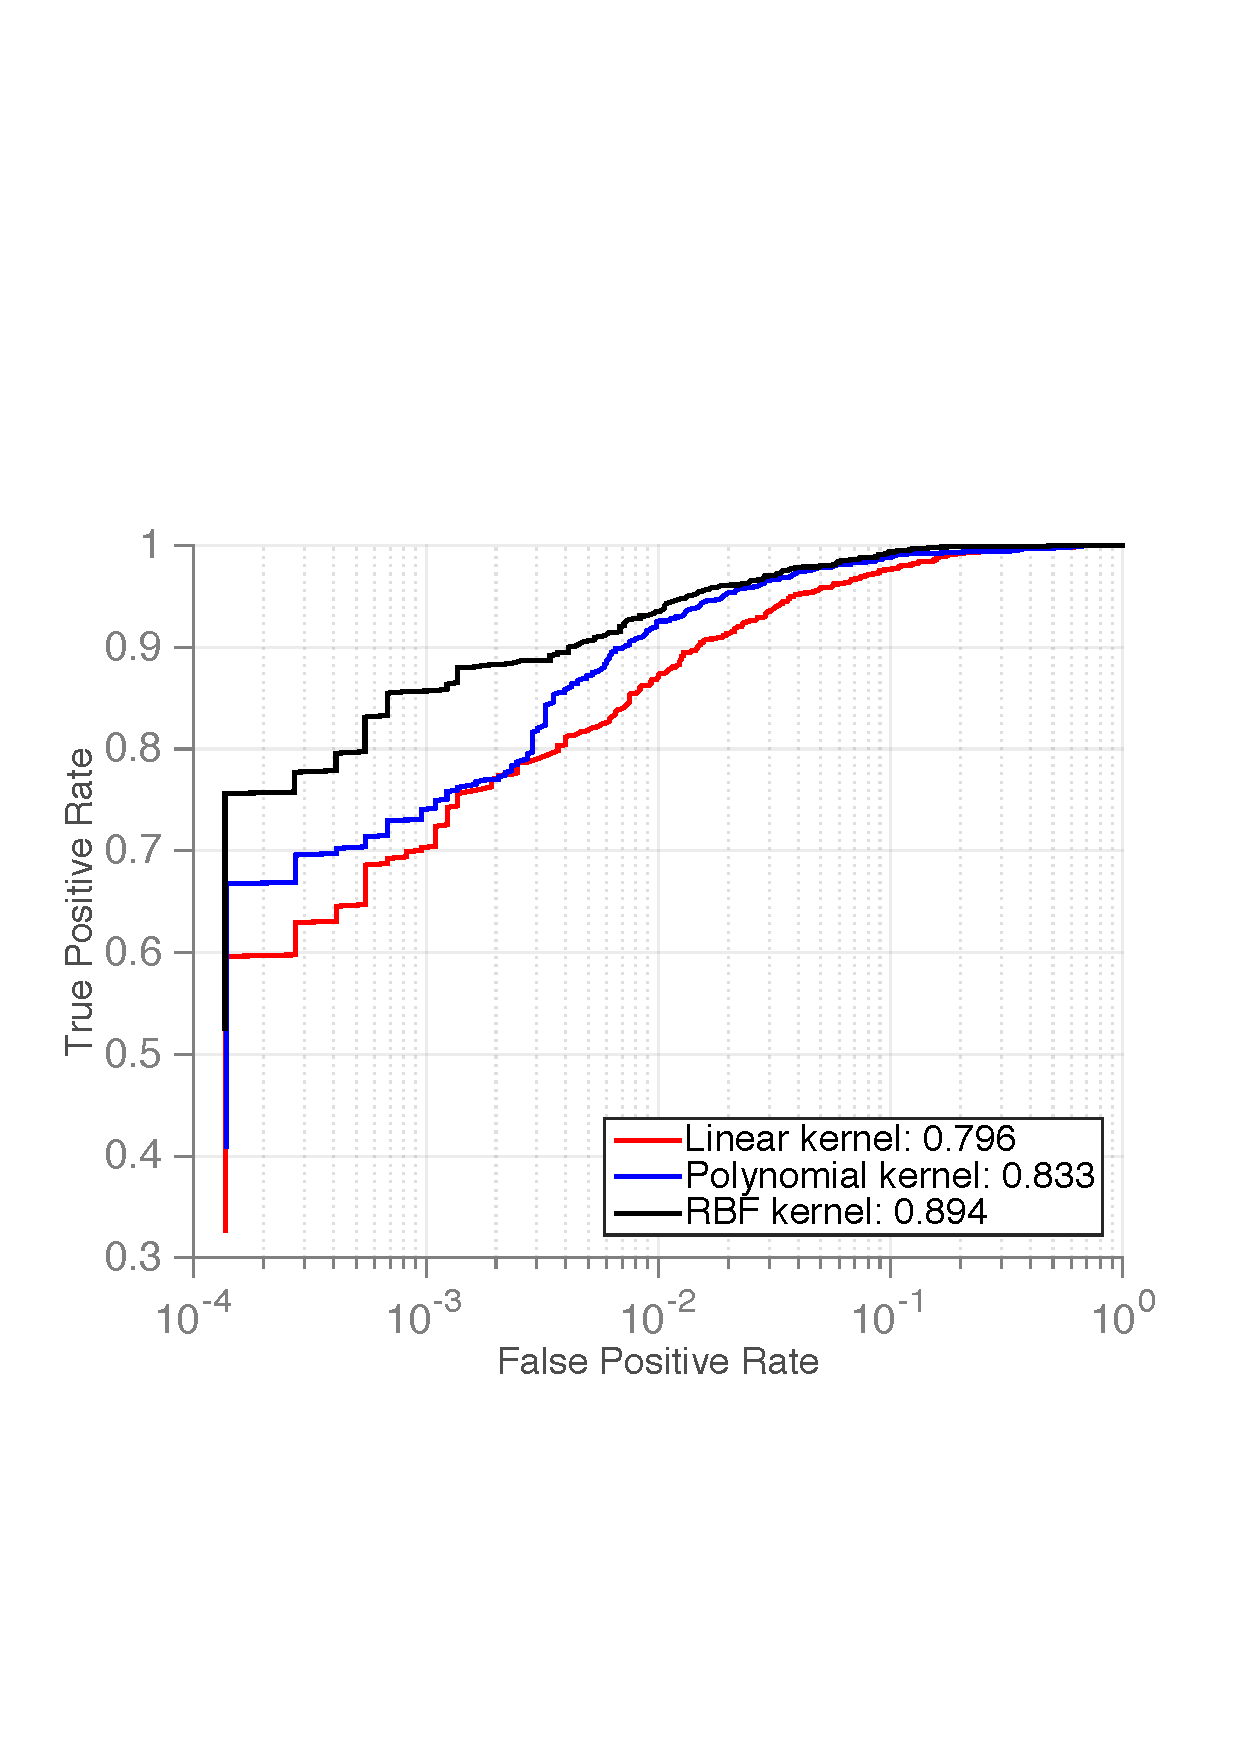
\includegraphics[width=2.5in]{figures/detection/svm-kernels-curve.pdf}
      		\label{fig:detection-svm-kernels}
      	}
    	\hfill
      	\subfigure[$\gamma$ parameter selection for the RBF kernel.]{
      		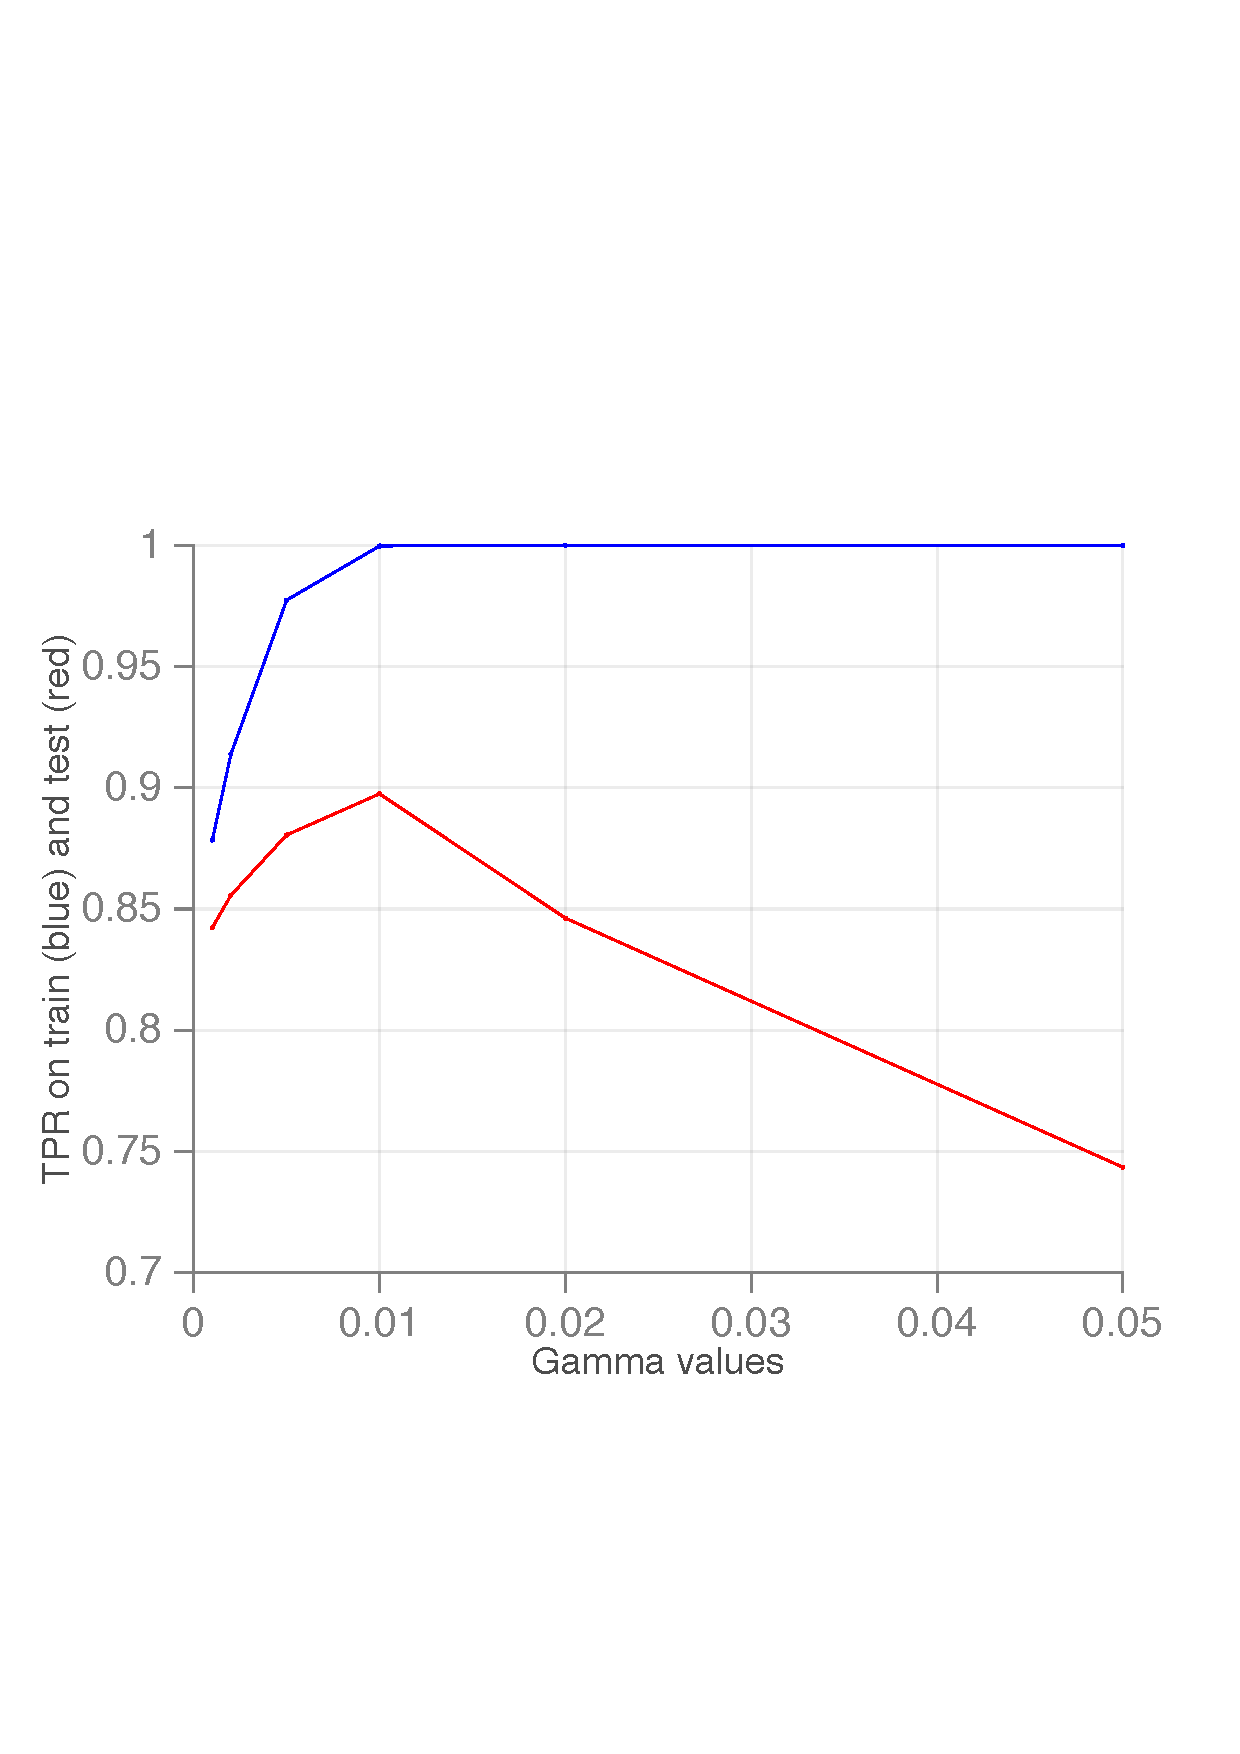
\includegraphics[width=2.5in]{figures/detection/svm-gamma-learningcurve.pdf}
      		\label{fig:detection-svm-gamma}
      	}
	\caption{Selecting the best parameters with ROC comparison and selecting parameters for SVM.}

  \end{figure}

  \subsection{Model selection and predictions}
    \textbf{Models comparison}:  Finally, we compare every candidate model with other classifiers plotting a ROC Curve averaged over 5-fold cross validation and a boxplot for each of them. The results are presented on Figure \ref{fig:detection-compare-roc-curve}. SVM with the RBF kernel on $X_{pca}$ gives the best performance with its ROC curve lying above the other classifiers and an average TPR reaching $0.911$. The second best classifier is Neural Networks on full-dimensionality data presenting the lowest variance over all methods. It worths pointing out the good performance of penalized Logistic Regression which is a very simple model. We did not expect much on the Gaussian Processes as we did not succeed to tune it a lot because of its sensitivity. However we are quite surprised about the Random Forest classifier which we would have expected to provide much better results as it is supposed to be particularly well fitted for such problems. We think that we might have not found the best settings for this classifier.

   \begin{figure}[ht]
       \center
      	\subfigure[Averaged ROC Curves of all our tuned classifiers.]{
      		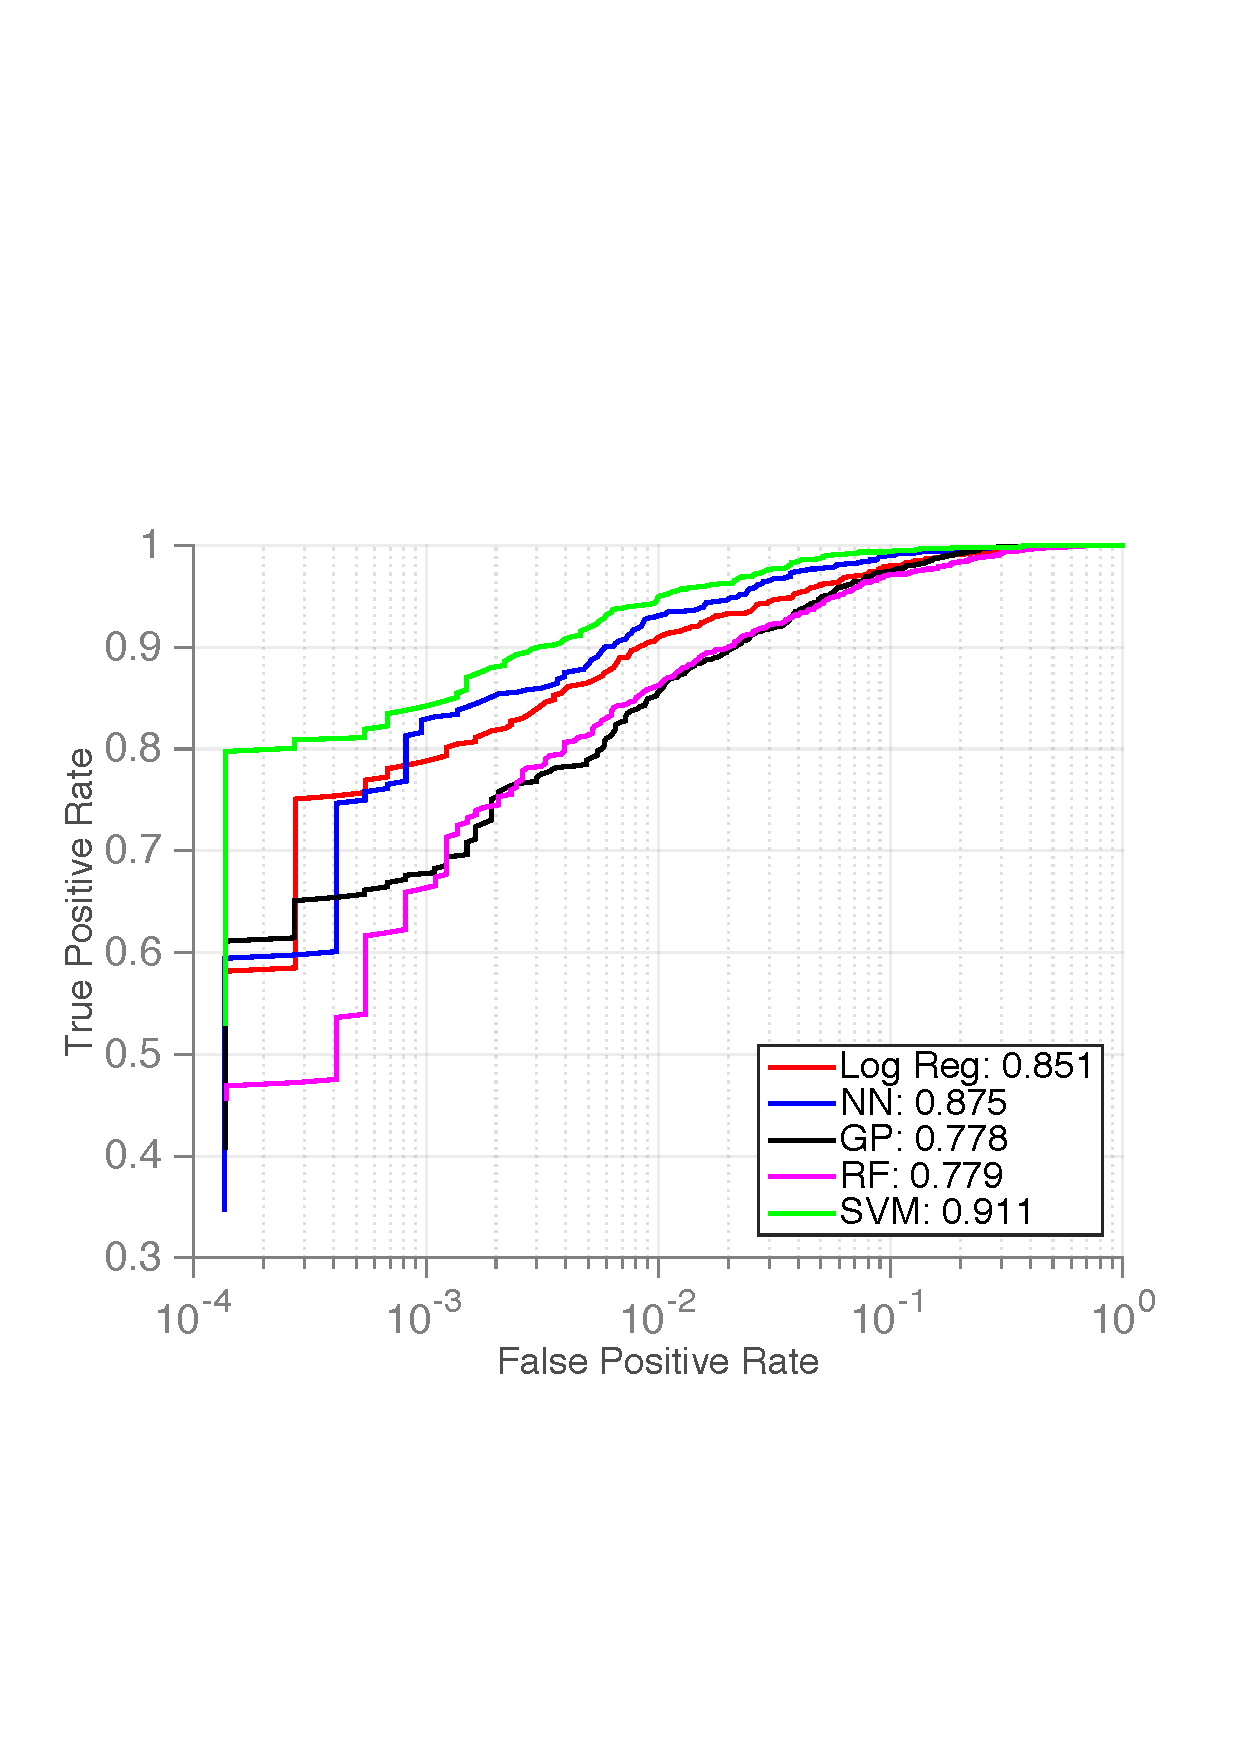
\includegraphics[width=2.5in]{figures/detection/compareall-5fold-curve.pdf}
      		\label{fig:detection-compare-roc-curve}
      	}
    	\hfill
	\subfigure[Boxplots of each classifier.]{
      		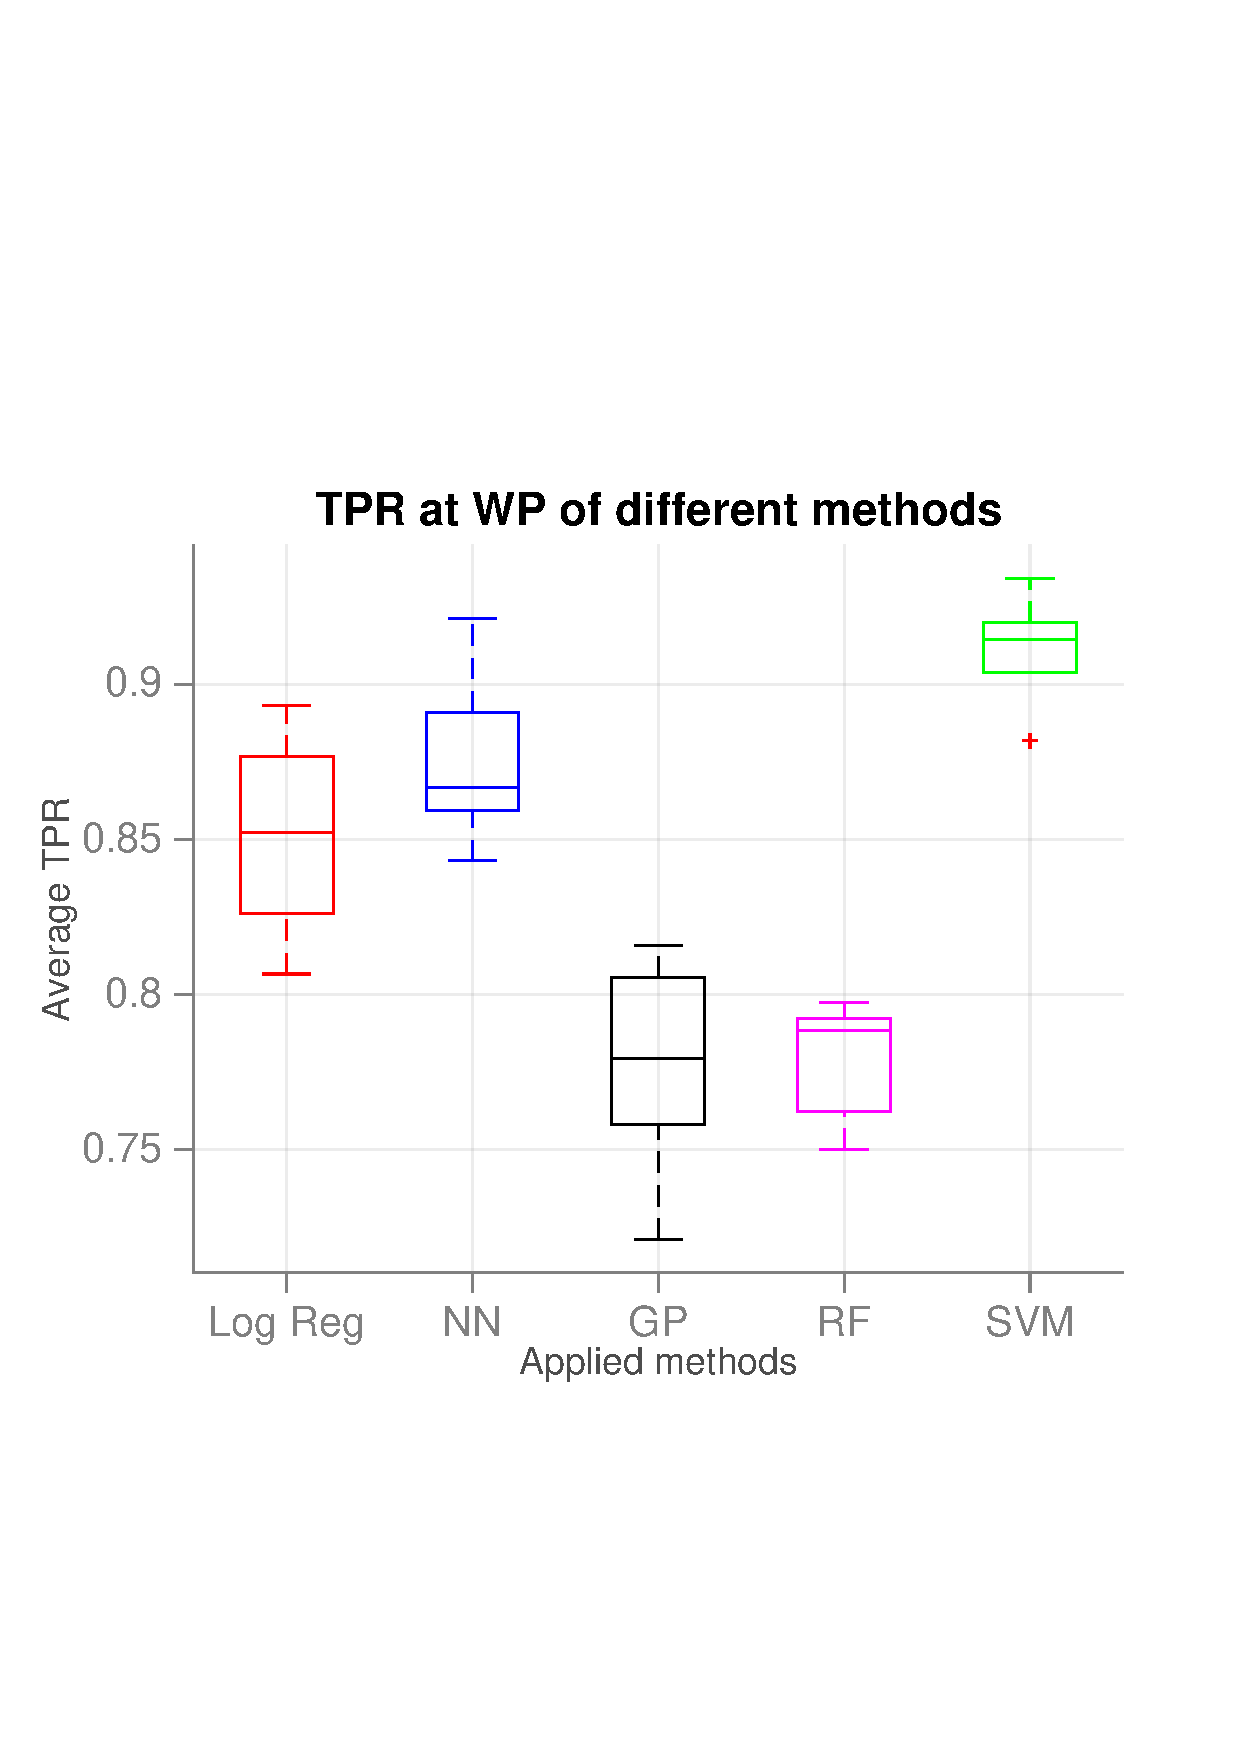
\includegraphics[width=2.5in]{figures/detection/compareall-5fold-boxplots.pdf}
      		\label{detection-compare-boxplot}
    	}
	\caption{Comparison of all models. SVM appear to provide the best performance.}
  \end{figure}

  \textbf{Predictions}: Hence, we produced our predictions for the given \texttt{X\_test} input data using the SVM classifier and wrote them in the mat file \texttt{personPred.mat}. We should underline that the predicted scores output from SVM are strongly split rather than smooth: our classifier seems to predict with high confidence, hence varying the threshold will not affect much our label predictions.

 \subsubsection*{Implementation details}
  When possible, we made use of parallel computations. In the song recommendation problem, we wrote a generic \texttt{evaluateMethod} function which runs any learning function passed and evaluates its performance over several random train / test splits. Our \texttt{diagnoseError} is used each time to visually verify the predictions. Predictions are generated in parallel from any predictor by the generic \texttt{generatePredictions.m} function. The ALS-WR algorithm is implemented in \texttt{alswr.m} and the parallel computation of Pearson's similarity coefficient in \texttt{computeSimilarityMatrix.m}. Sparse matrix representation made manipulation less straightforward and required us to learn a few new techniques.\\
  In the detection problem we updated the \texttt{fastROC} and \texttt{evaluateMultipleMethods} functions to versions based on cross-validation results. Our \texttt{kCVfastROC} function plots an averaged ROC curves with its $95\%$ confidence interval. We also wrote methods to find automatically the parameters of each methods and could re-use our generic \texttt{kFoldCrossValidation} function from project I.

\section{Summary}
  In the song recommendation problem, we reviewed several state of the art technique for model-based and collaborative filtering recommender systems. In most cases, we were not able to reproduce the results of the authors. However, we did gain valuable insight. We were able to beat the baseline by using a similarity-based approach. For strong generalization, artist-centered predictions worked best. Our main conclusion is that in presence of unstructured or other ``difficult'' data, simple approaches work best.\\
  In the detection problem, we first applied a PCA to reduce the dimensionality of our data. Then, we applied different classifiers and experimented with their parameters to improve their performance. Once having the optimal settings we could get, we compared them using ROC curves. Finally we selected SVM with RBF kernel for our predictions.

    \subsubsection*{Acknowledgments}
    We would like to thank Prof. Emtiyaz Khan and the teaching assistants for creating this project. It was a great opportunity for us to put in practice the machine learning techniques seen in class on real-world problems. We also would like to thank them for their availability throughout the semester. Thanks to our classmate Harris Jabbar for suggesting us to use Matlab's parallel processing capabilities.\\

    \begin{thebibliography}{99}
      % TODO: More references!

      % Papers
      \bibitem{alswr} Zhou, Y., Wilkinson, D., Schreiber, R., \& Pan, R., \textit{Large-scale parallel collaborative filtering for the netflix prize} (2008).
      \bibitem{long-tail-recommender} Park, Yoon-Joo, and Alexander Tuzhilin, \textit{The long tail of recommender systems and how to leverage it}.
      \bibitem{dropout} Srivastava N, Hinton G, Krizhevsky A, Sutskever I and Salakhutdinov R, \textit{Dropout: A Simple Way to Prevent Neural Networks from Overfitting}, in Journal of Machine Learning Research 15 (2014) 1929-1958.
      \bibitem{rocanalysis} Fawcett T, \textit{An introduction to ROC analysis}, in Pattern Recognition Letters 27 (2006) 861-874.
      \bibitem{cf-techniques-review} Xiaoyuan Su and Taghi M. Khoshgoftaar, \textit{A Survey of Collaborative Filtering Techniques} (2009)
      \bibitem{slope-one} Daniel Lemire, Anna Maclachlan, \textit{Slope One Predictors for Online Rating-Based Collaborative Filtering} (2007)
      \bibitem{cold-start-metrics} Pennock, Schein, Popescul and Ungar, \textit{Methods and Metrics for Cold-Start Recommendations} (2002)
      \bibitem{top-k-with-social-network} Xiwang Yang, Harald Steck,Yang Guo and Yong Liu, \textit{On Top-k Recommendation using Social Networks} (2012)

      % Code libraries
      \bibitem{piotrtoolbox} Doll'ar P, \textit{Piotr's Computer Vision Matlab Toolbox}
      \bibitem{gpmltoolbox} Rasmussen C and Williams C, \textit{Gaussian Processes for Machine Learning Toolbox}
      \bibitem{deeplearningtoolbox} Rasmus Berg Palm, \textit{Deep Learning Toolbox}
      \bibitem{libsvmtoolbox} Chang CC and Lin CJ, \textit{LIBSVM: A library for support vector machines}, in ACM Transactions on Intelligent Systems and Technology, vol. 2 (2011)
      \bibitem{gaussian-mixture-model-script} Mo Chen \textit{Variational Bayesian Inference for Gaussian Mixture Model}, on MathWorks File Exchange

    \end{thebibliography}

\end{document}
